\documentclass[11pt]{article}
\usepackage[utf8]{inputenc}
\usepackage[T1]{fontenc}
\usepackage{hyperref}
\usepackage{longtable,booktabs,array}
\usepackage{xcolor}
\usepackage{geometry}
\usepackage{fancyvrb}
\usepackage{framed}
\usepackage{tikz}
\usetikzlibrary{positioning,shapes,arrows.meta}
\usepackage{float}
\usepackage{setspace}

\geometry{margin=1in}
\setstretch{1.25}
\setlength{\parskip}{0.5em}

\providecommand{\tightlist}{%
  \setlength{\itemsep}{0pt}\setlength{\parskip}{0pt}}

\definecolor{shadecolor}{RGB}{248,248,248}
\newenvironment{Shaded}{\begin{snugshade}}{\end{snugshade}}

\begin{document}

\title{Architecture Report, Repository Audit, Standards Alignment \& Light Client Design}
\author{Julius Tranquilli \\ Lead Blockchain Developer at Webisoft Labs}
\date{}

\maketitle

\tableofcontents
\newpage

\section*{Overview}
\addcontentsline{toc}{section}{Overview}

This document provides an outline to early phase deliverables and design decisions for the Cardano-Cosmos IBC Bridge Incubator, as well as a summary of technical discussions that have taken place regarding the Hermes implementation, Mithril integration and limitations, and the relevant Cardano CIP pertaining to canonical chain state. This document should also serve as an ADR (Architecture Design Record) for implementations and considerations with respect to Mithril, CSMT, YACI store, and Hermes. We have successfully completed a repository audit, identified documentation gaps, validated IBC standards compatibility, designed light client architectures for both chains, and established the foundation for Hermes relayer integration, specifically the implementation details of the \texttt{ChainHandle} architecture. This document is designed to be as modular and discrete as possible so as to allow the reader to skip to points of interest, as there are significant technical details which warrant describing, but which may be overwhelming.

\section{Audit Report of Existing Codebase}
\label{audit-report-of-existing-codebase}

\subsection{Repository Structure}\label{repository-structure}

The codebase is organized into four main directories:

\textbf{Cardano Components} (\texttt{cardano/}):
\begin{itemize}
\item \textbf{Gateway (NestJS/TypeScript)}: Off-chain service providing gRPC endpoints for relayer communication, UTXO query orchestration, unsigned transaction building, and Mithril proof generation.
\item \textbf{Onchain validators (Aiken)}: Smart contracts implementing IBC primitives including client state storage, connection handshakes, channel management, and packet commitments.
\item \textbf{Offchain utilities (Deno/TypeScript)}: Transaction building helpers and UTXO analysis tools.
\end{itemize}

\textbf{Cosmos Components} (\texttt{cosmos/sidechain/}):
\begin{itemize}
\item \textbf{Cosmos SDK v0.50.6}: Application chain with custom light client modules.
\item \textbf{Mithril light client} (\texttt{x/clients/mithril/}): Implements ICS-02 interface for verifying Cardano state using Mithril's Stake-based Threshold Multisignatures.
\item \textbf{Cardano light client stub} (\texttt{x/clients/cardano/}): Placeholder for Tendermint-style verification (not yet production-ready).
\end{itemize}

\textbf{Relayer Components}:
\begin{itemize}
\item \textbf{Go Relayer} (\texttt{relayer/}): Forked from cosmos/relayer with Cardano ChainHandle implementation, currently using ibc-go v7.3.0.
\item \textbf{(Upcoming) Hermes Driver} (\texttt{hermes-driver/cardano-chain-handle/}): Rust-based ChainHandle trait implementation for integrating Cardano with the Hermes relayer, including Gateway gRPC client, CIP-1852 keyring, Ed25519 transaction signer, and IBC type conversions.
\end{itemize}

\textbf{CLI Infrastructure} (\texttt{caribic/}):
\begin{itemize}
\item \textbf{Rust CLI tool}: For orchestrating local development environment, managing Docker services, and providing user-facing bridge interaction commands. Seems a bit rusty at the moment but working to bring it back up to livelihood, particularly around the silent failure issues and infinite retries.
\end{itemize}

\subsection{Implementation Completeness and Audit Scope}
\label{implementation-completeness-assessment}

\textbf{Nature of This Audit}:

This audit differs from a traditional formal code audit since the existing repository is an early-stage implementation with a large number of TODOs, incomplete components, and actively deprecated modules (such as the Go relayer being replaced by Hermes). Rather than conducting an exhaustive line-by-line analysis of code that is either incomplete or scheduled for replacement, this audit focuses on:

  \begin{itemize}
\item \textbf{Architectural understanding}: Mapping the current system design and identifying which components are foundational versus transitional
\item \textbf{Gap identification}: Cataloging incomplete implementations and missing functionality
\item \textbf{Strategic planning}: Documenting design decisions and migration paths that will guide future development
\item \textbf{Standards alignment}: Assessing compatibility with IBC specifications and Cosmos SDK standards
  \end{itemize}

\textbf{Version Alignment}:

  \begin{itemize}
\item Go relayer (being deprecated) uses ibc-go v7.3.0 while sidechain uses v8.0.0
\item Cosmos SDK v0.50.6 currently in use; v0.52 available but not required for current functionality
\item Migration paths and compatibility considerations detailed in Section 3
  \end{itemize}

Given this early-stage status, the value of this audit lies in establishing a clear roadmap for completing the implementation rather than validating production-ready code. A formal security audit would be more appropriate once core implementations stabilize and TODOs are resolved.

\section{Documentation Gaps Identified and
Prioritized}\label{documentation-gaps-identified-and-prioritized}

\subsection{Documentation Status and Architecture Design Records}
\label{documentation-status-and-architecture-design-records}

This document addresses key architectural decisions and design rationale for the Cardano-Cosmos IBC Bridge. The following critical design decisions are documented in detail throughout this report:

\begin{enumerate}
\def\labelenumi{\arabic{enumi}.}
\tightlist
\item
  \textbf{Architecture Decision Records (Covered in This Document)}:

  \begin{itemize}
  \tightlist
  \item
    \textbf{Mithril-as-light-client design rationale}: Detailed in Section 5.2 (Cosmos Side: Mithril Light Client), including comparison with Tendermint light clients, CIP-0165 canonical state discussion, and CSMT alternative analysis.
  \item
    \textbf{Gateway architecture and relayer communication protocol}: Covered in Section 6.2 (Hermes--Gateway Integration Architecture) with detailed ChainHandle implementation in Section 4.3.
  \item
    \textbf{UTXO-based IBC state storage}: Documented in Section 5.4 (UTXO-Based State Storage Architecture) including Single Token Thread (STT) design, Channel UTXO structure, and indexer selection rationale (Kupo vs YACI Store).
\item
    \textbf{Hermes migration strategy}: Full ADR provided in Section 4 (ADR on Migration Strategy from Go Relayer to Hermes).
  \end{itemize}
\end{enumerate}

\subsection{Documentation Strategy}\label{documentation-strategy}

Given the early-stage nature of the implementation with numerous TODOs and components under active development or deprecation, significant documentation efforts would be premature at this time. Documentation should be treated as an ongoing effort that scales with implementation maturity.

\textbf{Recommended Approach}:

Defer detailed documentation (developer onboarding guides, operations manuals, contribution guidelines, deployment procedures) until the codebase reaches a more stable state. Focus current documentation efforts on:

  \begin{itemize}
\item Architectural Decision Records (ADRs) that capture design rationale for future reference
\item High-level system architecture and component interaction diagrams
\item Critical security considerations and trust assumptions
\item API contracts for stable interfaces
  \end{itemize}

As the implementation progresses toward completion and production readiness, documentation can be expanded to include operational guides, debugging procedures, and developer onboarding materials. This approach ensures documentation remains accurate and relevant rather than requiring constant updates to match evolving code.

\section{Compatibility Matrix for Cosmos SDK/ibc-go v10.x}
\label{compatibility-matrix-for-cosmos-sdkibc-go-v10.x}

\subsection{Current State}\label{current-state}

The Cardano IBC Incubator currently uses: - Cosmos SDK v0.50.6 in the
sidechain - ibc-go v8.0.0 in the sidechain - ibc-go v7.3.0 in the Go
relayer fork

\subsection{IBC-go v10.x Compatibility Assessment}
\label{ibc-go-v10.x-compatibility-assessment}

\textbf{ibc-go v10 Overview} (stable since March 2025, latest: v10.3.0):

ibc-go v10 represents a major protocol upgrade while maintaining
backward compatibility for v1 channels. The release introduces IBC v2 as
an opt-in enhancement alongside v1, requiring mandatory import path
updates due to Go semantic versioning but not forcing immediate v2
adoption. Key emphasis areas include improved packet lifecycle
management, enhanced light client flexibility, and ecosystem-wide
standardization.

\textbf{Major Changes Affecting Our Implementation}:

\textbf{1. Protocol \& Packet Lifecycle (IBC v2)}:
\begin{itemize}
\item IBC v2 protocol introduction with dual-stack support (v1 and v2 coexist).
\item Router-based module routing via port prefixes instead of just port IDs.
\item Simplified handshakes with no channel handshake callbacks required in v2 apps.
\item Packets route via client IDs, enabling easier non-Cosmos integrations (e.g., IBC Eureka for Ethereum).
\item Backward compatible: existing v1 channels continue to function without changes.
\end{itemize}

\textbf{2. Light Client Interface (ICS-02) Breaking Changes}:
\begin{itemize}
\item Updated \texttt{VerifyMembership} and \texttt{VerifyNonMembership} signatures with additional parameters.
\item Light client modules must update interface implementations to match new function signatures.
\item Explicit parameter updates required (e.g., add \texttt{exported.Localhost} to \texttt{AllowedClients} via upgrade handler).
\item New CosmWasm querier support for BLS aggregation/verification in 08-wasm light clients.
\item Enhanced flexibility for non-Tendermint consensus mechanisms (directly benefits Mithril implementation).
\end{itemize}

\textbf{3. Module Restructuring \& Import Changes}:
\begin{itemize}
\item \textbf{Mandatory import path updates}: All \texttt{/v7} imports must change to \texttt{/v10} (semantic versioning).
\item \textbf{Callbacks middleware}: Moved from separate module (\texttt{/apps/callbacks}) to core ibc-go.
\item \textbf{08-wasm light client}: Now releases as v10 (import: \texttt{/light-clients/08-wasm/v10}).
\item \textbf{ScopedKeeper removal}: Capability module deprecated, remove from keeper initialization.
\item \textbf{Legacy 02-client proposal handlers}: Removed from app routing (use \texttt{MsgRecoverClient} instead).
\end{itemize}

\textbf{4. Channel Upgrades (ICS-04)}:
\begin{itemize}
\item Support for upgrading channel parameters without closing the channel.
\item Governance proposals enable retrofitting fee middleware on existing channels.
\item New upgrade messages: \texttt{MsgChannelUpgradeInit}, \texttt{MsgChannelUpgradeAck}, etc.
\item Audited by Atredis (2024) for security compliance.
\end{itemize}

\textbf{5. Fee Middleware Improvements}:
\begin{itemize}
\item Enhanced relayer incentivization with channel upgrade compatibility.
\item Ability to add fee middleware to existing channels via governance.
\item Improved fee calculation and distribution logic.
\end{itemize}

\textbf{6. IBC v2-Specific Wiring Requirements}:
\begin{itemize}
\item New v2 router registration pattern: \texttt{porttypes.NewRouter().AddRoute(...)} for port prefixes.
\item Dual-stack wiring required: separate v1 (legacy) and v2 handlers in \texttt{app.go}.
\item Example: \texttt{ibcv2TransferStack} with \texttt{ibccallbacksv2.NewIBCMiddleware} for v2 transfer module.
\item v2 is opt-in but required for accessing new features (channel upgrades, simplified routing).
\end{itemize}

\textbf{7. Keeper \& Stack Changes}:
\begin{itemize}
\item Updated \texttt{NewKeeper} signatures: removed \texttt{legacySubspace} argument (pass \texttt{nil} for new chains).
\item IBC fee middleware must be removed from ICA controller/host stacks (use v2 equivalents).
\item All keeper initialization code must be updated to match new signatures.
\end{itemize}

\textbf{8. SDK \& CometBFT Dependencies}:
\begin{itemize}
\item Requires Cosmos SDK v0.50.x (breaking from v7's v0.47.x).
\item Requires CometBFT v0.38.x.
\item \textbf{Note}: ibc-go v9 was retracted; no v9 migration needed, go directly from v8 to v10.
\end{itemize}

\textbf{9. Deprecations \& Removals}:
\begin{itemize}
\item Removed legacy proposal types: \texttt{ClientUpdateProposal}, \texttt{UpgradeProposal} (replaced by \texttt{MsgRecoverClient}, \texttt{MsgIBCSoftwareUpgrade}).
\item Deprecated functions from v8 re-deprecated (scheduled for removal in v12).
\item API surface cleanup reduces technical debt but requires full test suite validation.
\end{itemize}

\textbf{Detailed Compatibility Status}:

\begin{longtable}{p{2.5cm}p{3.5cm}p{2.5cm}p{5.5cm}}
\toprule
\textbf{Component} & \textbf{Current Version} & \textbf{v10 Compatible} & \textbf{Required Changes} \\
\midrule
\endfirsthead
\toprule
\textbf{Component} & \textbf{Current Version} & \textbf{v10 Compatible} & \textbf{Required Changes} \\
\midrule
\endhead
\bottomrule
\endfoot
Cosmos Sidechain & SDK v0.50.6, ibc-go v8.0.0 & Partial & Import paths, v2 router wiring, keeper updates, SDK v0.50 alignment \\
\midrule
Mithril Light Client & ICS-02 compliant & Yes & Update interface signatures (minimal, already v10-style) \\
\midrule
Go Relayer & ibc-go v7.3.0 & No & Major refactor: v10 imports, v2 packet logic, keeper signatures, dual-stack routing \\
\midrule
Hermes Driver & N/A (external) & Yes & Hermes v1.9.0+ already v10 compatible \\
\midrule
Gateway & N/A (off-chain) & Yes & No IBC version dependency \\
\end{longtable}

\textbf{Migration Path to v10}:

\textbf{Sidechain Migration} (if/when needed):
\begin{itemize}
\item Update dependencies to ibc-go v10.3.0 and Cosmos SDK v0.50.x.
\item Update all import paths from \texttt{/v7} or \texttt{/v8} to \texttt{/v10}.
\item Wire v2 router in \texttt{app.go} for dual-stack operation (v1 and v2 coexist).
\item Update keeper initialization to remove deprecated parameters (\texttt{legacySubspace}, \texttt{ScopedKeeper}).
\item Update Mithril light client interface signatures for v10 ICS-02 changes.
\item Add \texttt{exported.Localhost} to \texttt{AllowedClients} via upgrade handler.
\item Run full test suite and validate v2 router, channel upgrades, and Mithril client compatibility.
\end{itemize}

\textbf{Go Relayer - NOT Migrating} (deprecating in favor of Hermes):
\begin{itemize}
\item Hypothetical migration effort would require: upgrading to v10.3.0, refactoring Cardano ChainHandle for v10 keeper signatures, implementing dual-stack v1/v2 routing, and extensive testing.
\item This represents significant ongoing maintenance burden (estimated 3-4 weeks initial work + indefinite upkeep).
\item \textbf{Decision}: Deprecate Go relayer fork, prioritize Hermes integration instead (see Section 4 for full rationale).
\end{itemize}

\textbf{Cosmos SDK v0.50 Alignment} (can be done alongside sidechain migration):
\begin{itemize}
\item Align with Cosmos SDK v0.50 breaking changes and module wiring updates.
\item Update CometBFT v0.38 dependencies and validate consensus compatibility.
\end{itemize}

\textbf{Recommendation}:

The Go relayer will not however be migrated to v10. Given the
substantial effort a hypothetical migration would require (v2 protocol
support, dual-stack wiring, keeper signature updates, plus ongoing
maintenance), we are deprecating the Go relayer fork entirely in favor
of Hermes integration. Hermes has been v10-compatible since early 2025
and provides superior performance, observability, and ecosystem support
with dramatically lower maintenance burden. The desired outcome is to
have Hermes be a ``drop-in'' replacement requiring no manual upkeep from
ibc-cardano-incubator maintainers.

For the sidechain, v10 migration provides access to channel upgrades,
improved fee middleware, and better light client flexibility that
directly benefits the Mithril implementation. This migration should be
scheduled based on project priorities and can be deferred until after
completing core Hermes ChainHandle implementation and initial end-to-end
testing on the current v8 stack.

\subsection{Cosmos SDK v0.52 Compatibility}
\label{cosmos-sdk-v0.52-compatibility}

Cosmos SDK v0.52 (latest stable) introduces:

\begin{itemize}
\item CometBFT v1.0 integration
\item Improved state management with IAVL v2
\item Enhanced module wiring with depinject improvements
\end{itemize}

\textbf{Compatibility}: The sidechain is compatible with v0.52 with minimal changes. Migration would primarily involve updating dependencies and adjusting for any deprecated APIs. This is a low-priority upgrade unless v0.52 provides critical security or performance improvements.

\subsection{Reference Sources}\label{reference-sources}

The details of this document are based on the following official
sources:

\begin{enumerate}
\def\labelenumi{\arabic{enumi}.}
\tightlist
\item
  \textbf{ibc-go v10 Migration Guide}:
  https://github.com/cosmos/ibc-go/blob/main/docs/migrations/v8-to-v10.md

  \begin{itemize}
  \tightlist
  \item
    Detailed breaking changes from v8.1 to v10
  \item
    Step-by-step migration instructions
  \item
    API surface changes and deprecated functions
  \end{itemize}
\item
  \textbf{ibc-go v10 Release Notes}:
  https://github.com/cosmos/ibc-go/releases/tag/v10.0.0

  \begin{itemize}
  \tightlist
  \item
    High-level feature overview
  \item
    Security audit reports (Atredis 2024)
  \item
    Dependency updates
  \end{itemize}
\item
  \textbf{ibc-go CHANGELOG}:
  https://github.com/cosmos/ibc-go/blob/main/CHANGELOG.md

  \begin{itemize}
  \tightlist
  \item
    Version-by-version change tracking (v10.0.0 through v10.3.0)
  \item
    Bug fixes and patch release notes
  \end{itemize}
\item
  \textbf{Cosmos SDK v0.50 Migration Guide}:
  https://github.com/cosmos/cosmos-sdk/blob/main/UPGRADING.md

  \begin{itemize}
  \tightlist
  \item
    Breaking changes from v0.47 to v0.50
  \item
    Module wiring updates
  \item
    CometBFT v0.38 integration notes
  \end{itemize}
\item
  \textbf{IBC Eureka Specifications} (for v2 protocol):
  https://github.com/cosmos/ibc/tree/main/spec/app/ics-030-middleware

  \begin{itemize}
  \tightlist
  \item
    IBC v2 router architecture
  \item
    Port prefix routing patterns
  \item
    Cross-ecosystem integration patterns
  \end{itemize}
\end{enumerate}

\section{Hermes Relayer Integration Strategy}
\label{hermes-relayer-integration-strategy}

\subsection{Rationale for Choosing Hermes}\label{rationale-for-choosing-hermes}

The project will transition from a forked Go relayer to Hermes, the Rust-based IBC relayer developed by Informal Systems. This decision was driven by several factors.

Hermes offers zero maintenance burden through its plugin architecture. Rather than maintaining a relayer fork and tracking upstream IBC protocol changes, the ChainHandle trait allows Cardano-specific logic to be cleanly isolated in a separate crate while core relayer functionality benefits from ongoing Informal Systems development. This architectural separation means that IBC protocol upgrades, performance improvements, and bug fixes in Hermes core automatically benefit the Cardano integration without requiring any Cardano-specific code changes.

From a production perspective, Hermes is battle-tested across dozens of Cosmos chains and represents the industry standard for IBC relaying. It provides superior performance for high-throughput scenarios, better observability and monitoring capabilities, and comprehensive operational tooling that alternatives lack. The active community support and corporate backing from Informal Systems ensure long-term viability and continuous improvement.

Alternative approaches (such as upgrading the Go relayer fork, which was on ibc-go v7.3.0 while the sidechain uses v8.0.0, building a custom relayer from scratch, or using less mature TypeScript implementations) would require significantly more development effort and create ongoing maintenance burdens while delivering inferior production capabilities. The Hermes integration represents a strategic investment in long-term operational excellence and ecosystem alignment.

\textbf{Implementation Progress}: We have scaffolded the \texttt{hermes-driver/cardano-chain-handle} Rust crate, stubbing the ChainHandle trait's 57 interface methods. The scaffolding includes Gateway gRPC client integration for querying Cardano state and submitting transactions, CIP-1852 compliant keyring implementation with mnemonic generation and key derivation, Ed25519 transaction signing for Cardano CBOR transactions, and type conversion helpers between Hermes IBC types and Gateway protobuf types. This foundational work establishes the adapter layer that translates between Hermes's chain-agnostic IBC operations and Cardano's UTXO-based architecture via the Gateway service.

\subsubsection{ChainHandle Implementation
Details}\label{chainhandle-implementation-details}

\textbf{ChainHandle vs ChainEndpoint Approach}:

Hermes provides two levels of integration for custom chains: the low-level ChainEndpoint trait (requiring direct blockchain interaction and Cosmos-like types) and the high-level ChainHandle trait (offering pure message-passing abstraction without Cosmos-specific types). We chose ChainHandle over ChainEndpoint because the latter would require deep SDK coupling with Cosmos-like types (Header, LightBlock, ConsensusState) ill-suited to Cardano's UTXO model, necessitate building CBOR parsing, UTXO indexing, and Plutus datum decoding from scratch in Rust despite minimal ecosystem support, duplicate all existing Gateway UTXO query logic by rewriting TypeScript code in Rust, force awkward type gymnastics to fit the UTXO model into account-based Tendermint abstractions, and create ongoing maintenance burden with every Cardano update requiring Rust code changes. In contrast, ChainHandle provides zero SDK coupling through pure interface abstraction with message-passing, maintains clean separation by keeping all UTXO/Aiken/Plutus/Cardano complexity isolated in the Gateway (TypeScript/NestJS), works naturally with async Gateway calls via crossbeam channels, simplifies testing by allowing easy Gateway mocking for unit tests, and establishes clear architectural boundaries where the Gateway serves as the Cardano expert while Hermes remains the IBC expert.

\textbf{The 56 ChainHandle Methods to Implement}:

The ChainHandle trait defines 57 methods (56 to implement, 1 has default
implementation):

\textbf{Category 1: Lifecycle \& Basic Operations} (5 methods)

\begin{itemize}
\item \texttt{new()} - Initialize ChainHandle
\item \texttt{id()} - Return chain ID
\item \texttt{shutdown()} - Cleanup resources
\item \texttt{health\_check()} - Health status check
\item \texttt{subscribe()} - Event subscription for monitoring
\end{itemize}

\textbf{Category 2: Transaction Submission} (2 methods)

\begin{itemize}
\item \texttt{send\_messages\_and\_wait\_commit()} - Submit transaction, wait for block inclusion
\item \texttt{send\_messages\_and\_wait\_check\_tx()} - Submit transaction, return immediately after mempool check
\end{itemize}

\textbf{Category 3: Key Management} (4 methods)

\begin{itemize}
\item \texttt{get\_signer()} - Get address/signer for transactions
\item \texttt{config()} - Return chain configuration
\item \texttt{get\_key()} - Get signing keypair
\item \texttt{add\_key()} - Add new key to keyring
\end{itemize}

\textbf{Category 4: Chain Metadata} (5 methods, includes 1 default)

\begin{itemize}
\item \texttt{version\_specs()} - IBC version information
\item \texttt{query\_balance()} - Query account balance
\item \texttt{query\_all\_balances()} - Query all token balances
\item \texttt{query\_denom\_trace()} - ICS-20 denomination trace info
\item \texttt{query\_application\_status()} - Current height and timestamp
\item \texttt{query\_latest\_height()} (default implementation) - Calls \texttt{query\_application\_status().height}
\end{itemize}

\textbf{Category 5: IBC Client Queries} (9 methods)

\begin{itemize}
\item \texttt{query\_clients()} - List all light clients
\item \texttt{query\_client\_state()} - Specific client state with optional proof
\item \texttt{query\_client\_connections()} - Connections for a client
\item \texttt{query\_consensus\_state()} - Consensus state at specific height
\item \texttt{query\_consensus\_state\_heights()} - All consensus state heights
\item \texttt{query\_upgraded\_client\_state()} - For client upgrade proposals
\item \texttt{query\_upgraded\_consensus\_state()} - For client upgrade proposals
\item \texttt{query\_commitment\_prefix()} - IBC commitment prefix (typically ``ibc'')
\item \texttt{query\_compatible\_versions()} - IBC connection version compatibility
\end{itemize}

\textbf{Category 6: IBC Connection Queries} (3 methods)

\begin{itemize}
\item \texttt{query\_connection()} - Specific connection with optional proof
\item \texttt{query\_connections()} - List all connections
\item \texttt{query\_connection\_channels()} - Channels for a connection
\end{itemize}

\textbf{Category 7: IBC Channel Queries} (4 methods)

\begin{itemize}
\item \texttt{query\_channels()} - List all channels
\item \texttt{query\_channel()} - Specific channel with optional proof
\item \texttt{query\_channel\_client\_state()} - Client for a channel
\item \texttt{query\_next\_sequence\_receive()} - Next receive sequence number
\end{itemize}

\textbf{Category 8: Light Client Building} (4 methods)

\begin{itemize}
\item \texttt{build\_header()} - Build client update header for remote chain
\item \texttt{build\_client\_state()} - Build initial client state
\item \texttt{build\_consensus\_state()} - Build consensus state from header
\item \texttt{check\_misbehaviour()} - Detect and report misbehavior evidence
\end{itemize}

\textbf{Category 9: Proof Building} (3 methods)

\begin{itemize}
\item \texttt{build\_connection\_proofs\_and\_client\_state()} - Connection existence proofs
\item \texttt{build\_channel\_proofs()} - Channel existence proofs
\item \texttt{build\_packet\_proofs()} - Packet commitment/receipt/ack proofs
\end{itemize}

\textbf{Category 10: Packet Commitment Queries} (4 methods)

\begin{itemize}
\item \texttt{query\_packet\_commitment()} - Single packet commitment with optional proof
\item \texttt{query\_packet\_commitments()} - All commitments for a channel
\item \texttt{query\_unreceived\_packets()} - Which packets destination hasn't received
\item \texttt{query\_packet\_receipt()} - Receipt for specific packet with optional proof
\end{itemize}

\textbf{Category 11: Packet Acknowledgement Queries} (3 methods)

\begin{itemize}
\item \texttt{query\_packet\_acknowledgement()} - Single acknowledgement with optional proof
\item \texttt{query\_packet\_acknowledgements()} - All acknowledgements for a channel
\item \texttt{query\_unreceived\_acknowledgements()} - Which acks source hasn't received
\end{itemize}

\textbf{Category 12: Event Queries} (2 methods)

\begin{itemize}
\item \texttt{query\_txs()} - Query transaction events by criteria
\item \texttt{query\_packet\_events()} - Query packet-specific events
\end{itemize}

\textbf{Category 13: Advanced Features} (9 methods)

\begin{itemize}
\item \texttt{query\_host\_consensus\_state()} - Host chain consensus state
\item \texttt{maybe\_register\_counterparty\_payee()} - ICS-29 fee middleware registration
\item \texttt{cross\_chain\_query()} - ICS-31 interchain queries
\item \texttt{query\_incentivized\_packet()} - ICS-29 fee information for packet
\item \texttt{query\_consumer\_chains()} - ICS-28 Cross-Chain Validation (CCV) consumer chains
\item \texttt{query\_upgrade()} - Channel upgrade information
\item \texttt{query\_upgrade\_error()} - Channel upgrade error details
\item \texttt{query\_ccv\_consumer\_id()} - CCV consumer chain identifier
\end{itemize}

\textbf{Implementation Strategy}:

For the Cardano ChainHandle, most methods will follow this pattern:

\begin{enumerate}
\item Translate Hermes IBC types to Gateway protobuf types
\item Make gRPC call to Gateway
\item Receive response from Gateway
\item Translate Gateway response back to Hermes types
\item Return to Hermes core
\end{enumerate}

\textbf{Example Implementation Flow}:

\begin{figure}[H]
\centering
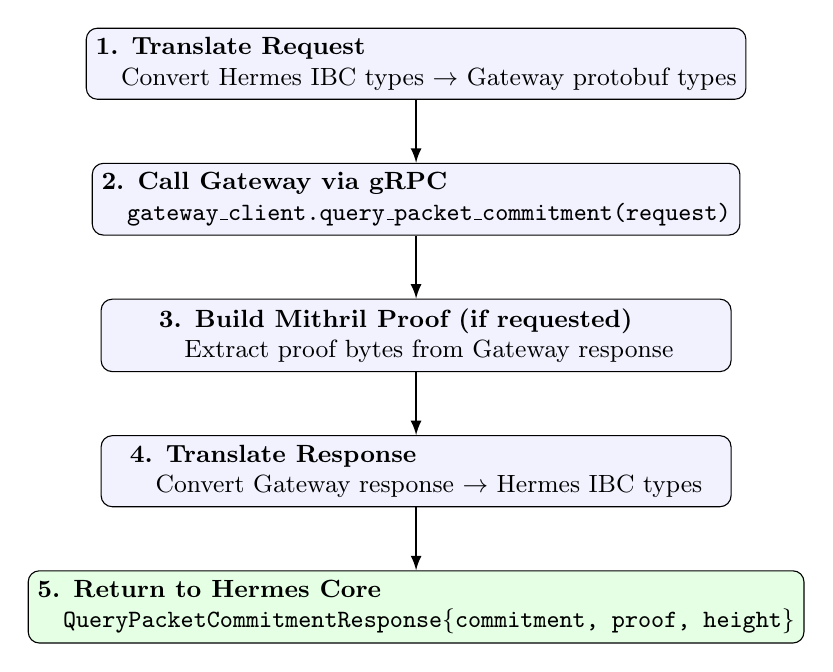
\begin{tikzpicture}[
  node distance=0.8cm,
  box/.style={rectangle, draw, rounded corners, align=left, font=\small, minimum width=8cm, minimum height=0.8cm, fill=blue!5},
  arrow/.style={->,>=latex,thick}
]
  \node[box] (step1) {\textbf{1. Translate Request}\\
    \quad Convert Hermes IBC types $\rightarrow$ Gateway protobuf types};
  
  \node[box, below=of step1] (step2) {\textbf{2. Call Gateway via gRPC}\\
    \quad \texttt{gateway\_client.query\_packet\_commitment(request)}};
  
  \node[box, below=of step2] (step3) {\textbf{3. Build Mithril Proof (if requested)}\\
    \quad Extract proof bytes from Gateway response};
  
  \node[box, below=of step3] (step4) {\textbf{4. Translate Response}\\
    \quad Convert Gateway response $\rightarrow$ Hermes IBC types};
  
  \node[box, below=of step4, fill=green!10] (step5) {\textbf{5. Return to Hermes Core}\\
    \quad \texttt{QueryPacketCommitmentResponse\{commitment, proof, height\}}};
  
  \draw[arrow] (step1) -- (step2);
  \draw[arrow] (step2) -- (step3);
  \draw[arrow] (step3) -- (step4);
  \draw[arrow] (step4) -- (step5);
\end{tikzpicture}
\caption{ChainHandle method implementation pattern: All 57 methods follow this adapter pattern, translating between Hermes and Gateway representations}
\label{fig:chainhandle-flow}
\end{figure}

The ChainHandle acts as a thin adapter layer, with all Cardano-specific
complexity (UTXO queries, transaction building, Aiken validators, datum
parsing) handled by the Gateway.

\section{Light Client and Proof Semantics}
\label{light-client-and-proof-semantics}

\subsection{IBC Light Client
Fundamentals}\label{ibc-light-client-fundamentals}

\paragraph{What Does a Light Client Do?}

A light client stores a trusted consensus state and provides two core functions:

\begin{enumerate}
\item Verify updates to the consensus state (tracking the remote chain's block headers and validator sets)
\item Verify packet commitments against the trusted root using Merkle proofs (proving that specific data exists or does not exist on the remote chain)
\end{enumerate}

\textbf{Major Interfaces}

IBC light clients must implement three primary interfaces as defined in
the \texttt{modules/core/exported} package of ibc-go:

\begin{enumerate}
\item
  \textbf{ClientState}: Contains all information needed to verify a
  ClientMessage and perform membership and non-membership proof
  verification of counterparty state. This includes properties that
  refer to the remote state machine, the light client type, and the
  specific light client instance.
\item
  \textbf{ConsensusState}: Tracks consensus data used for verification
  of client updates, misbehavior detection, and proof verification of
  counterparty state. This represents a snapshot of the remote chain's
  consensus at a specific height.
\item
  \textbf{ClientMessage}: Used for submitting block headers (single or
  batch) for client updates, and submission of misbehavior evidence
  using conflicting headers.
\end{enumerate}

\textbf{Handling Client Messages}

Light clients are updated by handling ClientMessage submissions
(typically from relayers via \texttt{MsgUpdateClient}). The 02-client
submodule's \texttt{UpdateClient} method processes client messages using
four key methods on the ClientState interface:

\begin{enumerate}
\def\labelenumi{\arabic{enumi}.}
\tightlist
\item
  \texttt{VerifyClientMessage}: Validates the format and cryptographic
  signatures of the submitted header(s).
\item
  \texttt{CheckForMisbehaviour}: Detects if the submitted headers
  contain evidence of misbehavior (e.g., double-signing).
\item
  \texttt{UpdateStateOnMisbehaviour}: Freezes the client if misbehavior
  is confirmed, preventing further updates.
\item
  \texttt{UpdateState}: Updates the ConsensusState with new block data
  if the header is valid and no misbehavior is detected.
\end{enumerate}

Additionally, ClientState includes methods for less frequent scenarios:

\begin{itemize}
\item \texttt{VerifyUpgradeAndUpdateState}: Updates the client when the remote chain upgrades its consensus protocol.
\item \texttt{CheckSubstituteAndUpdateState}: Replaces an expired client with a substitute client via governance proposal.
\end{itemize}

\textbf{Packet Commitment Verification}

Light clients provide verification for the IBC packet flow (send,
receive, acknowledge, timeout) using Merkle proofs against the trusted
root at standardized key paths defined in ICS-24 host requirements. The
connection keeper verifies packet state transitions by calling:

\begin{enumerate}
\def\labelenumi{\arabic{enumi}.}
\tightlist
\item
  \texttt{VerifyPacketCommitment}: Proves a packet was sent on the
  source chain (checked by destination when receiving).
\item
  \texttt{VerifyPacketAcknowledgement}: Proves a packet was acknowledged
  on the destination chain (checked by source).
\item
  \texttt{VerifyPacketReceiptAbsence}: Proves a packet was NOT received
  on the destination before timeout (checked by source for timeout
  processing).
\end{enumerate}

All of these rely on two fundamental verification methods: -
\texttt{VerifyMembership}: Proves inclusion (existence) of a value at a
given commitment path using a Merkle proof. -
\texttt{VerifyNonMembership}: Proves non-inclusion (non-existence) of a
value at a given commitment path.

The ICS-23 specification standardizes the Merkle proof format and
verification logic, ensuring interoperability across different chain
implementations.

\textbf{Governance Support Requirement}

Light client support in IBC is gated by on-chain governance. To create
client instances of a new client type, it must be added to the
\texttt{AllowedClients} parameter in the 02-client module via governance
proposal. For example, to add a new light client type, a parameter change proposal updates the \texttt{AllowedClients} list in the IBC subspace. The proposal specifies the key (\texttt{AllowedClients}) and the new value (an array including the new client type identifier, such as \texttt{09-mithril}, alongside existing types like \texttt{06-solomachine} and \texttt{07-tendermint}).

Once approved, relayers can create client instances by submitting
\texttt{MsgCreateClient} transactions with the new client type.

\subsubsection{How Standard IBC Light Clients Work:}
Tendermint/CometBFT
Reference}\label{how-standard-ibc-light-clients-work-tendermintcometbft-reference}

Before diving into our Mithril implementation, I just want to quickly explain how a typical IBC light client (Tendermint/CometBFT) achieves
both consensus verification and state verification with minimal trust
assumptions. I think this is also helpful for us to get a better grasp
of what the current limitations of Mithril and/or Cardano nodes are.

\paragraph{The Two-Layer Approach}

A standard IBC light client provides trustless verification through two sequential steps:

\begin{enumerate}
\item \textbf{Consensus Verification}: Prove that a particular block header is finalized by the correct validator set
\item \textbf{State Verification}: Prove that specific state (packet commitment, client state, etc.) existed in that finalized block
\end{enumerate}

\paragraph{Step 1: Consensus Verification (Trust the Block Header)}

The light client maintains:
\begin{itemize}
\item A trusted header at height \texttt{H\_trusted} (the last fully verified header)
\item Current validator set at \texttt{H\_trusted} with voting powers
\item Next validator set(s) for handling validator set rotations
\end{itemize}

To verify a new header at height \texttt{H\_target} (where
\texttt{H\_target\ \textgreater{}\ H\_trusted}):

The counterparty provides:
\begin{itemize}
\item Signed header at \texttt{H\_target} (including validator hash)
\item All intermediate headers from \texttt{H\_trusted+1} to \texttt{H\_target}
\item Validator sets (or validator set changes) for relevant heights
\item Commit containing 2/3+ precommit signatures for \texttt{H\_target} header
\end{itemize}

The light client performs:
\begin{enumerate}
\item \textbf{Signature Verification}: Check that each header is signed by >2/3 of the previous validator set's voting power
\item \textbf{Validator Set Progression}: Verify that validator set changes follow protocol rules
\item \textbf{Trusting Period Check}: Ensure that time elapsed since \texttt{H\_trusted} hasn't exceeded the trusting period (typically 2-3 weeks)
\item \textbf{Commit Verification}: Verify the commit for \texttt{H\_target} has >2/3 voting power from the validator set at \texttt{H\_target}
\end{enumerate}

If all checks pass -\textgreater{} the light client now trusts that
\texttt{H\_target} is finalized and canonical.

\paragraph{Step 2: State Verification (Prove Data Exists in Trusted Block)}

Once the header at \texttt{H\_target} is trusted, any Merkle proof rooted in that header is also trusted.

The counterparty provides:
\begin{itemize}
\item An ICS-23 Merkle proof showing that a specific key$\rightarrow$value pair existed in state at \texttt{H\_target}
\item The trusted header's \texttt{AppHash} (Cosmos SDK pre-v0.50) or \texttt{data\_hash} (v0.50+) serves as the Merkle root
\end{itemize}

The light client:
\begin{enumerate}
\item \textbf{Recompute Root}: Recomputes the Merkle root from the proof using the provided leaf, path, and siblings (ICS-23 IAVL proofs)
\item \textbf{Compare Against Trusted Root}: Compares the recomputed root against the \texttt{AppHash}/\texttt{data\_hash} in the trusted header
\end{enumerate}

If roots match -\textgreater{} the state is cryptographically proven to
have existed at the finalized block \texttt{H\_target}.

\paragraph{Understanding AppHash: The Canonical State Root}

\texttt{AppHash} (Application Hash) is the cornerstone of Tendermint's trustless state verification. It's a single 32-byte hash that represents the \textbf{entire application state} at a specific block height.
Loosely, we can say that to do this project properly, i.e., following the trustlessness principles of IBC,  we need to invent
a notion of \texttt{AppHash} for Cardano, analogous to the Cosmos
structure. Initially I thought I could sort of invent this abstraction
with my own on-chain implementation, but it's actually a chain-wide, and
node-level abstraction. This is what CIP-0165 is going to accomplish. We
can basically think of CIP-0165 as inventing Cardano's version of
AppHash.

\textbf{What AppHash Contains}:

\texttt{AppHash} is the root hash of an IAVL Merkle tree that stores all blockchain state:

\begin{itemize}
\item Account balances and nonces
\item Smart contract storage
\item IBC state (clients, connections, channels, packet commitments/acknowledgements/receipts)
\item Governance proposals and votes
\item Staking delegations and validator sets
\item Token supply and mint/burn records
\item Every key-value pair in the Cosmos SDK store
\end{itemize}

\textbf{How It Works}:

\begin{longtable}{p{4.5cm}p{10cm}}
\toprule
\multicolumn{2}{l}{\textbf{Block Header at Height 12345}} \\
\midrule
\endfirsthead
\toprule
\multicolumn{2}{l}{\textbf{Block Header at Height 12345}} \\
\midrule
\endhead
Height & 12345 \\
Timestamp & 2025-11-26T10:00:00Z \\
\textbf{AppHash} & \textbf{0xabcd1234...} (Root of IAVL Merkle tree containing all state) \\
ValidatorHash & 0x5678... (Hash of current validator set) \\
ConsensusHash & 0x9abc... \\
LastCommitHash & 0xdef0... \\
\midrule
\multicolumn{2}{l}{\textbf{Validator Signatures (>2/3 voting power required)}} \\
\midrule
Validator A & 30\% voting power, signs entire header including AppHash \\
Validator B & 25\% voting power, signs entire header including AppHash \\
Validator C & 20\% voting power, signs entire header including AppHash \\
... & (total >2/3 voting power) \\
\bottomrule
\end{longtable}

\textbf{Why This Is Critical}:

\begin{enumerate}
\def\labelenumi{\arabic{enumi}.}
\item
  \textbf{Canonical State Guarantee}: When \textgreater2/3 of validators
  sign a header with \texttt{AppHash\ =\ 0xabcd1234...}, they are
  cryptographically attesting that the application had state root
  \texttt{0xabcd1234...} at height 12345. There is NO ambiguity - all
  validators computed the exact same state and agreed on it.
\item
  \textbf{Trustless State Proofs}: Any Merkle proof that recomputes to
  \texttt{0xabcd1234...} is trustworthy because:

  \begin{itemize}
  \tightlist
  \item
    The proof is rooted in a hash signed by \textgreater2/3 validators
  \item
    You don't need to trust the relayer - you verify the Merkle path
    yourself
  \item
    You don't need to trust any indexer or full node - the proof is
    self-contained
  \end{itemize}
\item
  \textbf{Complete Security}: If a malicious relayer tries to provide a
  fake proof:

\begin{verbatim}
Relayer: "Here's proof that packet X exists"
Light Client: *recomputes Merkle root from proof*
Recomputed Root: 0x9999aaaa...
Trusted AppHash: 0xabcd1234...
Light Client: "REJECTED - roots don't match, proof is invalid"
\end{verbatim}
\end{enumerate}

\textbf{Cosmos SDK Version Evolution}:

\begin{itemize}
\tightlist
\item
  \textbf{Pre-v0.50}: Uses \texttt{AppHash} field in block headers
\item
  \textbf{v0.50+}: Uses \texttt{data\_hash} field (renamed for ABCI 2.0
  architecture, same concept)
\end{itemize}

Both represent the same thing: a single canonical hash of all
application state that all validators agree upon.

\textbf{The Mithril Challenge (Perhaps more like The Cardano Challenge)}:

This is what Mithril currently lacks (pre-CIP-0165). Mithril signers
cannot guarantee they're all signing the same UTxO set hash because: 
Cardano nodes may have slightly different views of the UTxO set at
signing timem, Network propagation delays mean different nodes see
transactions at different times, Mempool contents differ across nodes, 
and there's no deterministic ``snapshot point'' where all nodes agree to freeze
state

CIP-0165 aims to introduce this canonical state guarantee for Cardano,
enabling Mithril to have an equivalent to \texttt{AppHash} where all
signers provably sign the exact same ledger state at precise points.

\textbf{What This Enables for IBC}:

\begin{longtable}{p{4.5cm}p{10cm}}
\toprule
\textbf{Feature} & \textbf{How the Light Client Proves It} \\
\midrule
\endfirsthead
\toprule
\textbf{Feature} & \textbf{How the Light Client Proves It} \\
\midrule
\endhead
\bottomrule
\endfoot
\textbf{Consensus (finalized block)} & >2/3 validator signatures + correct validator set progression + trusting period checks \\
\midrule
\textbf{Packet existence \& ordering} & Merkle proof of packet commitment in \texttt{SendPacket}/\texttt{RecvPacket}/\texttt{WriteAck}/\texttt{WriteTimeout} events \\
\midrule
\textbf{Channel/Connection state} & Merkle proof of channel state, connection state, client state at specific paths \\
\midrule
\textbf{Token transfer (ICS-20) proof} & Merkle proof of denom trace + balance in escrow account or voucher mint/burn events \\
\end{longtable}

\paragraph{Trust Assumptions (Minimal)}

The Tendermint light client requires only two trust assumptions:

\begin{enumerate}
\item \textbf{Greater than 2/3 of validator set (by voting power) is honest} during the trusting period
\item \textbf{No long-range attack} (fork older than trusting period that rewrites history)
\end{enumerate}

That's it. No trusted third parties, no multisig committees, no oracles.

\textbf{Comparison: Standard Tendermint vs Current Mithril
Implementation}:

\begin{longtable}{p{3.5cm}p{5.5cm}p{5.5cm}}
\toprule
\textbf{Aspect} & \textbf{Cosmos IBC Tendermint Light Client} & \textbf{Current Cardano Mithril (Pre-CIP-0165)} \\
\midrule
\endfirsthead
\toprule
\textbf{Aspect} & \textbf{Cosmos IBC Tendermint Light Client} & \textbf{Current Cardano Mithril (Pre-CIP-0165)} \\
\midrule
\endhead
\bottomrule
\endfoot
\textbf{Consensus Verification Method} & >2/3 validator signatures on headers & STM aggregate signature from >51\% SPO stake \\
\midrule
\textbf{Same Consensus View Guarantee} & Yes (all validators sign identical header) & \textbf{No} (signers may snapshot slightly different ledger states) \\
\midrule
\textbf{Exact Same State Root} & Yes (\texttt{AppHash} in header represents single canonical state) & \textbf{No} (no guaranteed canonical state root at precise height) \\
\midrule
\textbf{State Proofs Possible} & Yes (ICS-23 Merkle proofs from \texttt{AppHash}) & \textbf{Not yet} (UTxO inclusion proofs not reliable, see Section 5.2.2) \\
\midrule
\textbf{Update Frequency} & Every block ($\sim$6 seconds) & Every Mithril snapshot ($\sim$6 hours on mainnet) \\
\midrule
\textbf{Trust Assumption} & >2/3 validators honest & >51\% SPO stake honest + trusted Gateway infrastructure for UTxO queries \\
\midrule
\textbf{State Storage Model} & IAVL Merkle tree in SDK KVStore & UTXO datums on Cardano blockchain \\
\midrule
\textbf{Finality} & Instant finality (BFT consensus) & Probabilistic finality + Mithril attestation (certificate lag) \\
\end{longtable}

\textbf{Why This Comparison Matters}:

The Tendermint light client represents the ``ideal'' that we're working
towards with Mithril. The key gap is the \textbf{canonical state
guarantee} - Tendermint validators all sign the exact same state root
(\texttt{AppHash}), enabling trustless state proofs. Mithril signers
currently cannot guarantee they're all signing the same UTxO set due to
network propagation delays and mempool differences.

\textbf{Path to Parity: CIP-0165 Canonical Ledger State}

Once CIP-0165 is implemented (see Section 5.2.2 for details), Mithril
signers will all sign the exact same state root at the same height -
exactly like a Tendermint header. At that point, Cardano will be able to
offer the same level of trust-minimized state proofs that Cosmos IBC has
had since 2021:

\begin{itemize}
\tightlist
\item
  \textbf{Before CIP-0165}: Transaction proofs (verified) + UTxO queries
  (trusted infrastructure)
\item
  \textbf{After CIP-0165}: Transaction proofs + UTxO inclusion proofs
  (both cryptographically verified)
\end{itemize}

This comparison establishes the baseline for understanding why our
current implementation has certain trust assumptions and how those will
be eliminated with protocol upgrades.

\subsubsection{IBC Light Client Interface}
Methods}\label{ibc-light-client-interface-methods}

\textbf{Complete Method Breakdown}:

IBC light clients must implement approximately 15-20 core methods across
three main interfaces (ClientState, ConsensusState, and ClientMessage).
The exact count varies slightly by ibc-go version, but the following
represents the standard ICS-02 interface:

\textbf{Category 1: ClientState Interface - Core Methods} (10 methods)

\begin{enumerate}
\def\labelenumi{\arabic{enumi}.}
\tightlist
\item
  \textbf{Client Lifecycle}:

  \begin{itemize}
  \tightlist
  \item
    \texttt{Initialize(ctx,\ clientID,\ clientState,\ consensusState)} -
    Initialize a new light client instance with genesis state
  \item
    \texttt{Status(ctx,\ clientStore)} - Returns client status: Active,
    Frozen, Expired, or Unknown
  \item
    \texttt{GetTimestampAtHeight(ctx,\ clientStore,\ height)} - Get
    timestamp for a specific height (for packet timeout verification)
  \end{itemize}
\item
  \textbf{Client Update \& Misbehavior} (4-step process):

  \begin{itemize}
  \tightlist
  \item
    \texttt{VerifyClientMessage(ctx,\ clientStore,\ cdc,\ clientMsg)} -
    Validate format and cryptographic signatures of submitted header(s)
  \item
    \texttt{CheckForMisbehaviour(ctx,\ clientStore,\ cdc,\ clientMsg)} -
    Detect if headers contain evidence of double-signing or equivocation
  \item
    \texttt{UpdateStateOnMisbehaviour(ctx,\ clientStore,\ cdc,\ clientMsg)}
    - Freeze client if misbehavior confirmed
  \item
    \texttt{UpdateState(ctx,\ clientStore,\ cdc,\ height,\ clientMsg)} -
    Update ConsensusState with new block data if valid
  \end{itemize}
\item
  \textbf{Proof Verification} (ICS-23):

  \begin{itemize}
  \tightlist
  \item
    \texttt{VerifyMembership(ctx,\ clientStore,\ cdc,\ height,\ delayTimePeriod,\ delayBlockPeriod,\ proof,\ path,\ value)}
    - Prove value exists at path
  \item
    \texttt{VerifyNonMembership(ctx,\ clientStore,\ cdc,\ height,\ delayTimePeriod,\ delayBlockPeriod,\ proof,\ path)}
    - Prove value does NOT exist at path
  \end{itemize}
\item
  \textbf{Client Upgrades \& Recovery}:

  \begin{itemize}
  \tightlist
  \item
    \texttt{VerifyUpgradeAndUpdateState(ctx,\ clientStore,\ cdc,\ newClient,\ newConsensus,\ proofUpgradeClient,\ proofUpgradeConsensus)}
    - Verify and execute client upgrade
  \item
    \texttt{CheckSubstituteAndUpdateState(ctx,\ clientStore,\ cdc,\ subjectClientStore,\ substitute)}
    - Replace expired client with substitute via governance
  \end{itemize}
\end{enumerate}

\textbf{Category 2: ClientState Interface - Helper Methods} (5-8
methods)

\begin{itemize}
\tightlist
\item
  \texttt{ClientType()} - Return client type identifier (e.g.,
  ``07-tendermint'', ``09-mithril'')
\item
  \texttt{GetLatestHeight()} - Get the latest height stored in client
  state
\item
  \texttt{Validate()} - Validate client state parameters (trust level,
  trusting period, etc.)
\item
  \texttt{GetProofSpecs()} - Return ICS-23 proof specs for this client
  type
\item
  \texttt{ZeroCustomFields()} - Zero out custom fields for deterministic
  marshalling
\item
  \texttt{ExportMetadata(clientStore)} - Export client-specific metadata
  for state export
\item
  \texttt{CheckHeaderAndUpdateState(ctx,\ clientStore,\ cdc,\ header)} -
  (DEPRECATED in v10, split into 4-step process above)
\item
  \texttt{CheckMisbehaviourAndUpdateState(ctx,\ clientStore,\ cdc,\ misbehaviour)}
  - (DEPRECATED in v10)
\end{itemize}

\textbf{Category 3: ConsensusState Interface} (3 methods)

\begin{itemize}
\tightlist
\item
  \texttt{ClientType()} - Return client type identifier (must match
  ClientState)
\item
  \texttt{GetTimestamp()} - Get timestamp of this consensus state (block
  time)
\item
  \texttt{ValidateBasic()} - Basic validation of consensus state fields
  (non-nil checks, format validation)
\end{itemize}

\textbf{Category 4: ClientMessage Interface} (2 methods)

\begin{itemize}
\tightlist
\item
  \texttt{ClientType()} - Return client type identifier
\item
  \texttt{ValidateBasic()} - Basic validation of message fields
\end{itemize}

\textbf{Category 5: Height Interface} (6 methods)

\begin{itemize}
\tightlist
\item
  \texttt{GetRevisionNumber()} - Get revision number (for chain
  upgrades)
\item
  \texttt{GetRevisionHeight()} - Get revision height (block height)
\item
  \texttt{Compare(other)} - Compare two heights (-1, 0, 1)
\item
  \texttt{LT(other)} - Less than comparison
\item
  \texttt{LTE(other)} - Less than or equal comparison
\item
  \texttt{GT(other)} - Greater than comparison
\item
  \texttt{GTE(other)} - Greater than or equal comparison
\item
  \texttt{Increment()} - Increment height by 1
\item
  \texttt{Decrement()} - Decrement height by 1
\item
  \texttt{IsZero()} - Check if height is zero value
\item
  \texttt{String()} - String representation
\end{itemize}

\textbf{Implementation Requirements by Client Type}:

\textbf{For Mithril Light Client}
(\texttt{cosmos/sidechain/x/clients/mithril/}):

\textbf{Mithril Light Client State Structures}:

\begin{longtable}{p{4cm}p{3cm}p{7.5cm}}
\toprule
\textbf{Structure} & \textbf{Field} & \textbf{Description} \\
\midrule
\endfirsthead
\toprule
\textbf{Structure} & \textbf{Field} & \textbf{Description} \\
\midrule
\endhead
\textbf{ClientState} & ChainId & Cardano network identifier (mainnet, preprod) \\
(ICS-02 interface) & TrustLevel & Minimum stake threshold (e.g., 51\%) \\
 & TrustingPeriod & Max time before client expires without update \\
 & UnbondingPeriod & Cardano unbonding period ($\geq$21 days) \\
 & MaxClockDrift & Allowed clock drift between chains \\
 & FrozenHeight & Height at which client was frozen (zero if active) \\
 & LatestHeight & Latest verified height \\
 & GenesisKey & Genesis certificate public key (root of trust) \\
\midrule
\textbf{ConsensusState} & Timestamp & Certificate sealed\_at timestamp \\
(Mithril certificate) & CertificateHash & Mithril certificate hash \\
 & MerkleRoot & Snapshot merkle root from certificate \\
 & Epoch & Cardano epoch number \\
 & AggregateKey & SPO aggregate verification key \\
\midrule
\textbf{MithrilHeader} & Certificate & Full certificate from Mithril aggregator \\
(Client update) & TrustedHeight & Previously verified height \\
\bottomrule
\end{longtable}

\textbf{Key ClientState Methods}:
\begin{itemize}
\item \texttt{VerifyMembership}: Verify Mithril certificate + CBOR datum extraction
\item \texttt{UpdateState}: Store new Mithril certificate as ConsensusState
\item \texttt{CheckForMisbehaviour}: Check for conflicting Mithril certificates at same height
\end{itemize}

\textbf{For Cardano Tendermint Light Client}
(\texttt{cosmos/sidechain/x/clients/cardano/}):

Similar structure but adapted for Tendermint-style consensus
verification instead of Mithril STM signatures.

\textbf{Key Differences from Standard Tendermint Client}:

\begin{longtable}{p{3.5cm}p{5.5cm}p{5.5cm}}
\toprule
\textbf{Aspect} & \textbf{Standard Tendermint} & \textbf{Mithril Client} \\
\midrule
\endfirsthead
\toprule
\textbf{Aspect} & \textbf{Standard Tendermint} & \textbf{Mithril Client} \\
\midrule
\endhead
\bottomrule
\endfoot
\textbf{Consensus Verification} & 2/3+ validator signatures on headers & STM aggregate signature from >51\% SPO stake \\
\midrule
\textbf{Update Frequency} & Every block ($\sim$6 seconds) & Every Mithril snapshot ($\sim$6 hours) \\
\midrule
\textbf{Proof Structure} & IAVL Merkle proofs & MithrilWrappedProof (certificate + tx proof + UTXO metadata) \\
\midrule
\textbf{State Storage} & IAVL tree in SDK KVStore & UTXO datums on Cardano blockchain \\
\midrule
\textbf{Finality Model} & Instant finality (BFT) & Probabilistic finality + Mithril attestation \\
\midrule
\textbf{Trust Assumptions} & 1/3+ honest validators & >51\% honest stake (economic security) \\
\end{longtable}

\textbf{Implementation Status}:

Both Mithril and Cardano light clients implement the full ICS-02
interface. The key implementation work involves:

\begin{enumerate}
\def\labelenumi{\arabic{enumi}.}
\tightlist
\item
  \textbf{Certificate Verification Logic}: Mithril-specific STM
  signature verification (already implemented in
  \texttt{cosmos/sidechain/x/clients/mithril/crypto/})
\item
  \textbf{CBOR Datum Parsing}: Extracting IBC state from UTXO datums
  (implemented in proof\_verifier.go)
\item
  \textbf{Path Mapping}: Converting ICS-24 paths to datum locations
  (implemented, see Section 5.3)
\item
  \textbf{Merkle Proof Verification}: Transaction inclusion in Mithril
  snapshots (partially implemented, awaiting Mithril proof format spec)
\end{enumerate}

\subsection{Cardano Side: ICS-07 Tendermint Light Client}\label{cardano-side-ics-07-tendermint-light-client}

The Cardano light client implementation (\texttt{cosmos/sidechain/x/clients/cardano/}) provides ICS-02 interface support for verifying Cardano state from Cosmos chains, though it remains in early development and not yet production-ready. The implementation stores Tendermint block headers and validator sets, verifies Ed25519 signatures, and implements ICS-23 proof verification for UTXO-based state. The verification flow decodes MithrilWrappedProof structures from relayers, validates Mithril certificates with SPO signatures and stake thresholds, extracts Merkle roots, verifies transaction inclusion, parses CBOR datums from UTXOs, maps ICS-24 paths to datum locations, and compares extracted values against expected values. Current limitations include incomplete Merkle proof verification (awaiting Mithril proof format specification), certificate lag requiring retry logic, and UTXO spending race conditions between query and verification. This implementation serves as the counterpart to the Mithril light client, enabling bidirectional IBC communication between Cardano and Cosmos chains.

\subsection{Cosmos Side: Mithril Light Client}\label{cosmos-side-mithril-light-client}

\textbf{Status}: Core verification complete, integration tested with
mocked data.

\textbf{Architecture} (\texttt{cosmos/sidechain/x/clients/mithril/}):

\textbf{Mithril Certificate to ICS-23 Proof Adaptation}:

The Mithril client adapts Mithril's certificate-based trust model to ICS-23's proof verification interface by wrapping the base MithrilCertificate with additional proof data:

\begin{figure}[H]
\centering
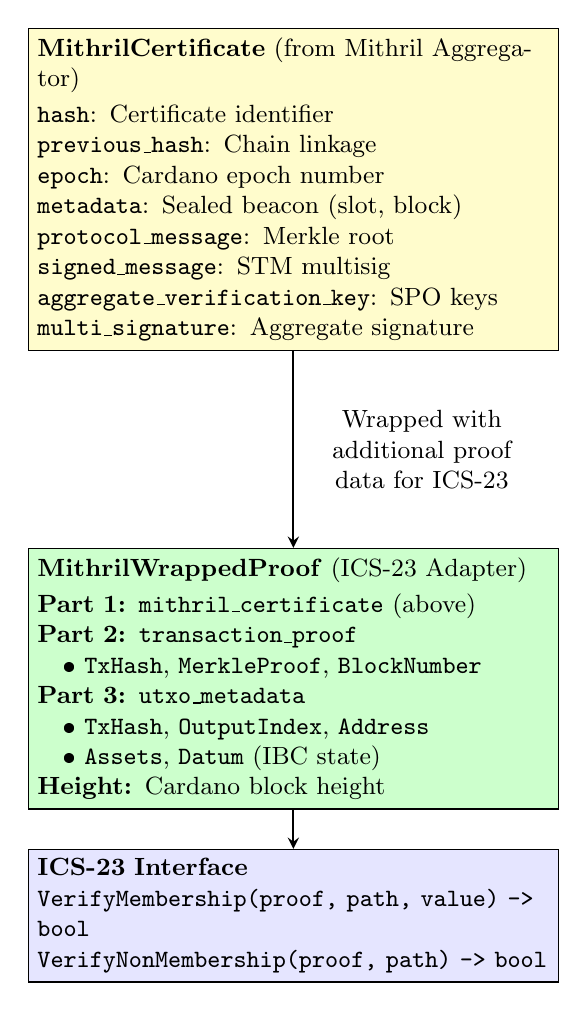
\begin{tikzpicture}[
  node distance=0.3cm,
  box/.style={rectangle, draw, text width=6.5cm, align=left, font=\small},
  component/.style={rectangle, draw, fill=blue!10, text width=6.5cm, align=left, font=\small, minimum height=1.2cm},
  arrow/.style={->, >=stealth, thick}
]

% MithrilCertificate box
\node[box, fill=yellow!20] (cert) {
  \textbf{MithrilCertificate} (from Mithril Aggregator)\\[2pt]
  \texttt{hash}: Certificate identifier\\
  \texttt{previous\_hash}: Chain linkage\\
  \texttt{epoch}: Cardano epoch number\\
  \texttt{metadata}: Sealed beacon (slot, block)\\
  \texttt{protocol\_message}: Merkle root\\
  \texttt{signed\_message}: STM multisig\\
  \texttt{aggregate\_verification\_key}: SPO keys\\
  \texttt{multi\_signature}: Aggregate signature
};

% MithrilWrappedProof box
\node[box, fill=green!20, below=2.5cm of cert] (wrapped) {
  \textbf{MithrilWrappedProof} (ICS-23 Adapter)\\[2pt]
  \textbf{Part 1:} \texttt{mithril\_certificate} (above)\\
  \textbf{Part 2:} \texttt{transaction\_proof}\\
  \quad • \texttt{TxHash}, \texttt{MerkleProof}, \texttt{BlockNumber}\\
  \textbf{Part 3:} \texttt{utxo\_metadata}\\
  \quad • \texttt{TxHash}, \texttt{OutputIndex}, \texttt{Address}\\
  \quad • \texttt{Assets}, \texttt{Datum} (IBC state)\\
  \textbf{Height:} Cardano block height
};

% Arrow from cert to wrapped with label
\draw[arrow] (cert.south) -- node[right, font=\small, text width=3cm, align=center] {Wrapped with additional proof data for ICS-23} (wrapped.north);

% ICS-23 interface box
\node[component, below=0.5cm of wrapped] (ics23) {
  \textbf{ICS-23 Interface}\\
  \texttt{VerifyMembership(proof, path, value) -> bool}\\
  \texttt{VerifyNonMembership(proof, path) -> bool}
};

% Arrow from wrapped to ICS-23
\draw[arrow] (wrapped.south) -- (ics23.north);

\end{tikzpicture}
\caption{Mithril Certificate Adaptation for ICS-23 Proof Verification}
\label{fig:mithril-wrapped-proof}
\end{figure}

\textbf{Verification Steps}:

\begin{enumerate}
\item \textbf{Certificate Chain Validation}:
\begin{itemize}
\item Retrieve previous certificates from client store.
\item Verify each certificate's \texttt{previous\_hash} links correctly.
\item Ensure no gaps in certificate chain.
\end{itemize}

\def\labelenumi{\arabic{enumi}.}
\tightlist
\item
  \textbf{STM Signature Verification}:

  \begin{itemize}
  \tightlist
  \item
    Fetch Cardano epoch's stake distribution from client state.
  \item
    Verify aggregate signature using SPO public keys and stakes.
  \item
    Ensure stake threshold (e.g., 51\%) is met for quorum.
  \end{itemize}
\item
  \textbf{Height Consistency}:

  \begin{itemize}
  \tightlist
  \item
    Verify certificate's sealed beacon height matches proof's claimed
    height.
  \item
    Ensure height is not regressed (monotonically increasing).
  \end{itemize}
\item
  \textbf{Transaction Inclusion}:

  \begin{itemize}
  \tightlist
  \item
    Extract Merkle root from certificate's protocol message.
  \item
    Verify transaction hash is included in Merkle tree (using provided
    proof).
  \end{itemize}
\item
  \textbf{State Extraction}:

  \begin{itemize}
  \tightlist
  \item
    Parse UTXO datum as CBOR.
  \item
    Navigate to ICS-24 path location in datum structure.
  \item
    Extract value and compare with expected value.
  \end{itemize}
\end{enumerate}

\textbf{ICS-23 Compatibility}:
  \begin{itemize}
\item Implements required \texttt{VerifyMembership} and \texttt{VerifyNonMembership} methods.
\item Supports all ICS-24 standard paths (clients, connections, channels, packet commitments, acknowledgements, and receipts).
\item Error handling for missing proofs, invalid signatures, and malformed datums.
  \end{itemize}

\textbf{State Verification Challenges and Solutions}:

The \texttt{VerifyMembership} and \texttt{VerifyNonMembership} methods represent the core of IBC's trustless state verification, but their implementation for Cardano faces unique challenges due to fundamental differences between Cardano's UTXO model and Cosmos's account-based state machine. These challenges and our approaches are discussed throughout this document:

\textbf{Canonical State Problem (CIP-0165)}: As detailed in Section 5.0.1 (Tendermint vs Mithril comparison) and Section 5.2.2 (UTxO Inclusion Proofs limitation), Mithril currently cannot provide cryptographic proofs of UTxO inclusion because SPOs cannot guarantee they're all signing the exact same UTxO set. CIP-0165 (Canonical Ledger State) aims to solve this by introducing a mechanism for Cardano nodes to compute and agree upon a canonical ledger state hash at specific points, analogous to Tendermint's \texttt{AppHash}. Until CIP-0165 is implemented, our \texttt{VerifyMembership} relies on transaction proofs (cryptographically verified) combined with UTxO queries (trusted Gateway infrastructure).

\textbf{UTXO Indexing and Query Layer}: The \texttt{utxo\_metadata} component of MithrilWrappedProof requires efficient UTXO queries to locate IBC state. Section 5.4.2 discusses our indexer selection (Kupo vs YACI Store), where we chose Kupo for its lightweight design and NFT-friendly querying that aligns perfectly with our Single Token Thread (STT) architecture. The STT design (Section 5.4.1) simplifies state verification by using a unique NFT to identify canonical state, eliminating ambiguity about which UTXO represents "current" state, a critical simplification for \texttt{VerifyMembership} operations.

\textbf{Alternative Proof Approaches (CSMT)}: Section 5.2.2 also discusses Paolino Veronelli's CSMT (Compact Sparse Merkle Tree) UTxO proof engine as a potential future optimization. While CSMT provides efficient cryptographic proofs of UTxO inclusion/exclusion at specific chainpoints, it doesn't solve the canonical state agreement problem that CIP-0165 addresses. CSMT is complementary: once CIP-0165 provides canonical state roots, CSMT could optimize proof generation against those roots, potentially improving \texttt{VerifyMembership} performance.

\textbf{Trust Model Trade-offs}: The current implementation accepts a trust assumption on Gateway infrastructure for UTxO queries (mitigated by relayers running their own Cardano nodes) in exchange for immediate functionality. This pragmatic approach allows IBC operations to proceed while the Cardano ecosystem develops canonical state guarantees. The \texttt{VerifyMembership} and \texttt{VerifyNonMembership} methods are architected to seamlessly upgrade to fully trustless verification once CIP-0165 is available, requiring only updates to the proof verification logic without changes to the ICS-23 interface.

\subsubsection{Mithril Certificate Technical Details}\label{mithril-certificate-technical-details}

I want to clarify first that, while we can create on-chain abstractions to digest and verify Mithril certificates, it's not totally clear whether this is needed at this point in time, specifically with respect to ICS-23. Mithril certificates are produced through a multi-step process involving Cardano SPOs. At the beginning of each Cardano epoch, the Mithril aggregator reads the stake distribution from the Cardano chain, computes protocol parameters (quorum threshold, security parameter, stake eligibility), and allows participating SPOs to register as signers with ephemeral keys. Every six hours on mainnet, the aggregator syncs to the latest immutable Cardano block, computes a UTXO set snapshot by extracting all UTXOs, building a Merkle tree, computing the merkle root representing the entire UTXO set, and packaging this into a ProtocolMessage containing the merkle root and beacon (epoch, immutable file number). The aggregator then creates a certificate candidate linking to the previous certificate (forming a chain), includes metadata about registered SPOs and timestamps, computes the signed message (hash of all certificate data), and broadcasts the candidate to all registered signers.

Each SPO signer receives the certificate candidate, verifies its legitimacy by checking that the beacon points to real chain state and the snapshot matches their local view, generates an STM signature using their secret key weighted by stake, and submits their individual signature to the aggregator. The aggregator collects individual signatures, checks if quorum is reached (typically greater than 51% stake), aggregates signatures using STM into a single compact signature, and creates the final certificate with the aggregate signature. Each certificate points to the previous certificate via \texttt{previous\_hash}, forming a tamper-evident chain from the current certificate back through all previous certificates to the genesis certificate, preventing modification of old certificates without breaking the chain and allowing verification of lineage back to genesis.

Currently, verifying a Mithril certificate involves six cryptographic checks performed by the light client. First, certificate chain verification retrieves the previous certificate from the client store and verifies that \texttt{hash(previous\_cert) == current\_cert.previous\_hash} to ensure correct certificate lineage and prevent fake certificate chains. Second, genesis signature verification confirms the certificate links to the genesis certificate (the root of trust bootstrapped and distributed out-of-band), ensuring all valid certificates link to the same genesis using the genesis public key. Third, signed message reconstruction recomputes the message that was signed from certificate data (including merkle root, beacon, metadata) to ensure the certificate hasn't been tampered with after signing. Fourth, aggregate verification key (AVK) extraction parses the \texttt{aggregate\_verification\_key} from the certificate, which is the combined public key of all eligible signers weighted by stake, representing the collective signing authority of participating SPOs. Fifth, STM signature verification parses the \texttt{multi\_signature} and cryptographically verifies \texttt{STM\_Verify(AVK, signed\_message, signature)}—this is the core of Mithril's efficiency, providing O(1) verification time regardless of the number of signers, where a single signature check proves hundreds of SPOs signed rather than checking each individually. Sixth, stake threshold checking computes the total stake of all eligible signers and the signed stake of SPOs who actually signed, verifying that \texttt{(signed\_stake * 100) >= (total\_stake * threshold)}, typically requiring greater than 51% stake participation for security, and rejecting certificates below the threshold even if cryptographically valid.

\begin{figure}[H]
\centering
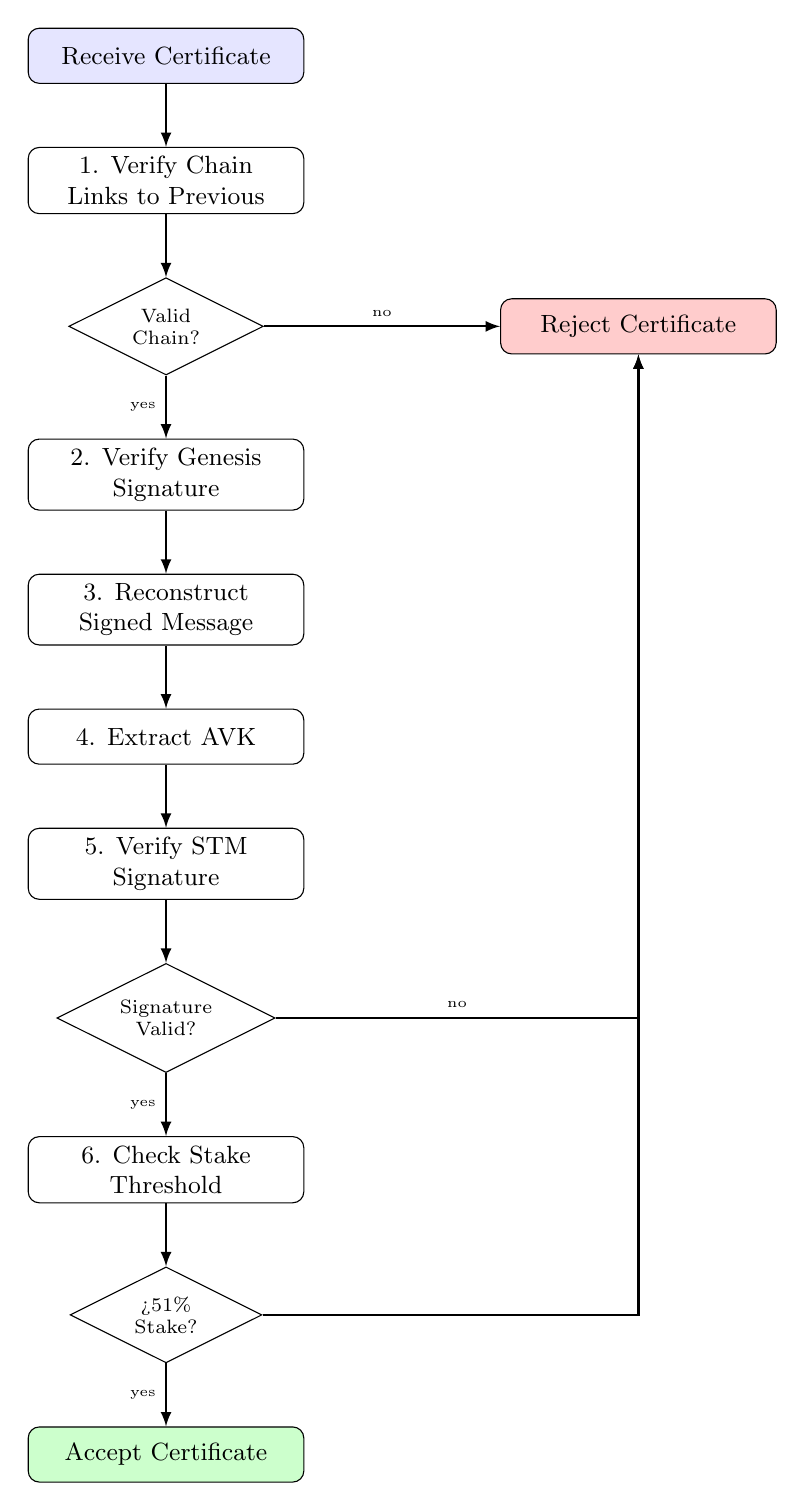
\begin{tikzpicture}[
  node distance=0.8cm and 1.5cm,
  box/.style={rectangle, draw, rounded corners, align=center, font=\small, minimum width=3.5cm, minimum height=0.7cm},
  decision/.style={diamond, draw, align=center, font=\scriptsize, minimum width=2cm, minimum height=1.2cm, aspect=2},
  arrow/.style={->,>=latex,thick}
]
  % Nodes
  \node[box, fill=blue!10] (start) {Receive Certificate};
  \node[box, below=of start] (step1) {1. Verify Chain\\Links to Previous};
  \node[decision, below=of step1] (check1) {Valid\\Chain?};
  \node[box, below=of check1] (step2) {2. Verify Genesis\\Signature};
  \node[box, below=of step2] (step3) {3. Reconstruct\\Signed Message};
  \node[box, below=of step3] (step4) {4. Extract AVK};
  \node[box, below=of step4] (step5) {5. Verify STM\\Signature};
  \node[decision, below=of step5] (check2) {Signature\\Valid?};
  \node[box, below=of check2] (step6) {6. Check Stake\\Threshold};
  \node[decision, below=of step6] (check3) {>51\%\\Stake?};
  \node[box, below=of check3, fill=green!20] (accept) {Accept Certificate};
  \node[box, right=3cm of check1, fill=red!20] (reject) {Reject Certificate};
  
  % Arrows
  \draw[arrow] (start) -- (step1);
  \draw[arrow] (step1) -- (check1);
  \draw[arrow] (check1) -- node[left,font=\tiny] {yes} (step2);
  \draw[arrow] (check1) -- node[above,font=\tiny] {no} (reject);
  \draw[arrow] (step2) -- (step3);
  \draw[arrow] (step3) -- (step4);
  \draw[arrow] (step4) -- (step5);
  \draw[arrow] (step5) -- (check2);
  \draw[arrow] (check2) -- node[left,font=\tiny] {yes} (step6);
  \draw[arrow] (check2.east) -| node[above,font=\tiny,pos=0.25] {no} (reject);
  \draw[arrow] (step6) -- (check3);
  \draw[arrow] (check3) -- node[left,font=\tiny] {yes} (accept);
  \draw[arrow] (check3.east) -| (reject);
\end{tikzpicture}
\caption{Mithril Certificate Verification Algorithm: Six-step validation process with early rejection on failure}
\label{fig:mithril-verification}
\end{figure}

\textbf{MithrilWrappedProof Structure}:

The ICS-23 adapter wraps Mithril certificates with additional proof data in a three-part structure:

\begin{longtable}{p{4cm}p{3.5cm}p{7cm}}
\toprule
\textbf{Component} & \textbf{Field} & \textbf{Purpose} \\
\midrule
\endfirsthead
\toprule
\textbf{Component} & \textbf{Field} & \textbf{Purpose} \\
\midrule
\endhead
\textbf{Part 1:} & Certificate & Proves: "Cardano blockchain had state X at height Y" \\
\textbf{Mithril Certificate} & (MithrilCertificate) & Contains SPO signatures, stake distribution, merkle root \\
\midrule
\textbf{Part 2:} & TxHash & Transaction hash \\
\textbf{Transaction Proof} & MerkleProof & Hex-encoded merkle path from snapshot root to transaction \\
 & BlockNumber & Block height \\
 & \textit{Purpose} & \textit{Proves: "Transaction H is included in the certified snapshot"} \\
\midrule
\textbf{Part 3:} & TxHash & Transaction hash \\
\textbf{UTXO Metadata} & OutputIndex & Output index in transaction \\
 & Address & UTXO address \\
 & Assets & Token amounts (map) \\
 & Datum & Hex-encoded CBOR datum containing IBC state \\
 & \textit{Purpose} & \textit{Proves: "UTXO's datum contains value V at path P"} \\
\midrule
\textbf{Height} & Height & Cardano block height this proof is for \\
\bottomrule
\end{longtable}

\textbf{Verification Flow with Wrapped Proof}:

When the Cosmos sidechain receives a MithrilWrappedProof:

\begin{enumerate}
\def\labelenumi{\arabic{enumi}.}
\tightlist
\item
  \textbf{Decode Proof}: Unmarshal protobuf bytes into
  MithrilWrappedProof structure
\item
  \textbf{Verify Certificate}: Run 6-step certificate verification
  algorithm (chain -\textgreater{} genesis -\textgreater{} message
  -\textgreater{} AVK -\textgreater{} signature -\textgreater{} stake
  threshold)
\item
  \textbf{Verify Transaction Inclusion}: Use
  TransactionProof.MerkleProof to prove TransactionProof.TxHash is in
  the snapshot's Merkle tree with root from
  Certificate.ProtocolMessage.MerkleRoot
\item
  \textbf{Parse CBOR Datum}: Decode UtxoMetadata.Datum from hex-encoded
  CBOR to structured data
\item
  \textbf{Map ICS-24 Path}: Convert IBC path (e.g.,
  ``clients/07-tendermint-0/clientState'') to datum location (e.g.,
  datum.state.client\_state)
\item
  \textbf{Extract and Compare}: Navigate datum structure to extract
  value, compare with expected value
\end{enumerate}

This three-part proof structure (Certificate + Transaction + UTXO)
enables the Cosmos sidechain to verify Cardano state without running a
full Cardano node, while maintaining cryptographic security through SPO
stake-based signatures.

\textbf{Known Limitation: UTxO Inclusion Proofs and CIP-0165}

As highlighted in the Tendermint vs Mithril comparison (Section 5.0.1),
Mithril currently has a critical limitation: it cannot provide
cryptographic proofs of UTxO inclusion in the certified ledger state.
While Mithril can certify transaction inclusion (via transaction Merkle
proofs), it cannot cryptographically prove that a specific UTxO exists
in the ledger at the moment of certification.

\textbf{Root Cause}: Mithril signers (SPOs) cannot guarantee they are
all signing the exact same UTxO set because different Cardano nodes may
have slightly different views of the ledger at signing time due to
network propagation delays, mempool differences, and block production
timing. This prevents consensus on a single canonical UTxO set hash.

\textbf{Impact on Our Implementation}: Since Cardano IBC stores all
state (clients, connections, channels, packet commitments) in UTxO
datums, the \texttt{MithrilWrappedProof} currently includes UTxO
metadata alongside transaction proofs, but the UTxO inclusion itself is
not cryptographically verified. We verify ``this transaction happened''
but trust Gateway infrastructure (Kupo/Ogmios) to provide correct UTxO
state.

\textbf{Trust Assumption}: This introduces reliance on Gateway's Cardano
node infrastructure. An attacker compromising the Gateway could provide
fake UTxO data even with valid Mithril certificates. The risk is
mitigated by relayers running their own nodes, but prevents pure
trustless light client verification.

\textbf{Solution: CIP-0165 Canonical Ledger State}
(https://github.com/cardano-foundation/CIPs/pull/1083)

This Cardano Improvement Proposal introduces:

\begin{enumerate}
\item \textbf{Canonical Ledger State}: Mechanism for Cardano nodes to compute and agree upon a canonical ledger state hash at specific points
\item \textbf{Deterministic Snapshot Triggers}: Configuration to trigger Mithril snapshots at precise, predetermined points (epoch boundaries, specific slots)
\end{enumerate}

Once implemented (expected 6-12 months based on CIP review timelines),
Mithril signers will all sign the exact same UTxO set - achieving the
same canonical state guarantee as Tendermint headers with
\texttt{AppHash}.

\paragraph{Post-CIP-0165 Benefits}

True trustless verification becomes possible:

\begin{itemize}
\item Cosmos chains verify Cardano UTxO state with only Mithril certificates
\item No trusted Cardano node required
\item Eliminates Gateway trust assumption
\item Parity with Tendermint light client security model
\end{itemize}

\textbf{Current Mitigation}: Transaction proofs (cryptographically
verified) + UTxO queries (trusted infrastructure) + relayer-operated
nodes for fraud detection + regular Gateway audits.

\textbf{Alternative Approach: CSMT UTxO Proof Engine}

Following a discussion with Paolino Veronelli, we investigated CSMT (Compact Sparse Merkle Tree) as a potential solution for UTxO inclusion/exclusion proofs. Paolino is building a generic UTxO proof engine that tracks the full UTxO set and issues cryptographic proofs of inclusion/exclusion. His implementation has great performance: "fast enough to keep up with 800 UTxO changes a second over 3.5M stored UTxO" and "loads preprod UTxOs in 1h (3.5M)." The system is designed to provide proofs of UTxO at address completeness, allowing services to cryptographically justify their claims about UTxOs rather than requiring blind trust.

In Paolino's architecture, services would "host a utxo-csmt to collect proofs to corroborate their claims," while other parties run their own utxo-csmt instances and "stream (chainpoint, merkle-tree-root, signature of them)." Mithril is positioned as one possible signer stream: "mithril could be the best one to follow, if/when ready," though he notes "do not plan to use Mithril for now," instead leaving "trust decision to the user on which (potentially multiple) stream of signatures to follow."

\textbf{Assessment for IBC Integration}: CSMT provides a solid reusable layer for UTxO inclusion/exclusion proofs at specific chainpoints, including address-level completeness if needed. It offers a clean mechanism to prove "given this root for slot S, here is a proof that this UTxO is (or isn't) in the set." However, it does not solve the fundamental IBC challenge: determining which root/chainpoint is canonical and who attests to it. As Paolino acknowledges, "about multi-signature over the merkle tree roots, mithril is obviously the right tech," and divergent views "aren't an issue as long as parties 'stream' (chainpoint, merkle-tree-root, signature...)."

In other words, CSMT helps once you've chosen a snapshot and a signer stream you trust, but it doesn't provide the stake-weighted, protocol-level canonicalization or snapshot-coordination that an IBC light client requires. CSMT is complementary to Mithril/CIP-0165 rather than a replacement: CIP-0165 provides canonical state agreement, while CSMT could provide efficient proof generation against that canonical state. We should keep up to date with Paolino's work as a potential future optimization layer once the canonical state problem is resolved.

\subsection{Interface Implementation}
Summary}\label{interface-implementation-summary}

\textbf{How Our Light Clients Fulfill IBC Requirements}

Both the Cardano Tendermint light client (on Cosmos) and the Mithril
light client (on Cosmos) implement the required IBC interfaces as
follows:

\textbf{ClientState Interface Implementation}:
\begin{itemize}
\item \texttt{cosmos/sidechain/x/clients/cardano/client\_state.go}: Implements ClientState for Cardano with Tendermint-style consensus verification.
\item \texttt{cosmos/sidechain/x/clients/mithril/client\_state.go}: Implements ClientState for Mithril with STM-based consensus verification.
\item Both include \texttt{VerifyMembership} and \texttt{VerifyNonMembership} methods for ICS-23 proof verification against the respective trusted roots.
\end{itemize}

\textbf{ConsensusState Interface Implementation}:
\begin{itemize}
\item \texttt{cosmos/sidechain/x/clients/cardano/consensus\_state.go}: Stores Tendermint block headers and validator sets.
\item \texttt{cosmos/sidechain/x/clients/mithril/consensus\_state.go}: Stores Mithril certificates with SPO stake distribution and aggregate verification keys.
\end{itemize}

\textbf{ClientMessage Handling}:
\begin{itemize}
\item \texttt{cosmos/sidechain/x/clients/cardano/update.go}: Processes Tendermint header updates with Ed25519 signature verification.
\item \texttt{cosmos/sidechain/x/clients/mithril/update.go}: Processes Mithril certificate updates with STM multisignature verification.
\item Both implement the four-step update process: VerifyClientMessage, CheckForMisbehaviour, UpdateStateOnMisbehaviour, and UpdateState.
\end{itemize}

\textbf{Proof Verification Methods}:

\textbf{For Cardano Tendermint Light Client}:
\begin{itemize}
\item \texttt{VerifyMembership}: Decodes MithrilWrappedProof, verifies Mithril certificate chain, checks transaction inclusion via Merkle proof, parses CBOR datum, maps ICS-24 path to datum location, extracts and compares values.
\item \texttt{VerifyNonMembership}: Same process but verifies absence of value at specified path.
\end{itemize}

\textbf{For Mithril Light Client}:

Granted, as Mithril is experimental and under active development, and there is also a pending relevant CIP, it's not totally clear which of the IBC light client interface methods will be delegated to Mithril functionalities, so we may take the separation of responsibilities in this domain with a grain of salt for now.

\begin{itemize}
\item \texttt{VerifyMembership}: Validates certificate chain links, verifies STM aggregate signature with stake threshold, checks height consistency, verifies transaction inclusion in Merkle tree, extracts state from UTXO datum.
\item \texttt{VerifyNonMembership}: Validates certificate and proves value does not exist at path (datum field absent or null).
\end{itemize}

\textbf{ICS-24 Path Support}:

Both light clients support all standard IBC paths for packet flow verification:

\begin{itemize}
\item \texttt{clients/\{client-id\}/clientState}: Client configuration and parameters
\item \texttt{clients/\{client-id\}/consensusStates/\{height\}}: Historical consensus states for proof verification
\item \texttt{connections/\{connection-id\}}: Connection handshake state
\item \texttt{channelEnds/ports/\{port-id\}/channels/\{channel-id\}}: Channel handshake state
\item \texttt{commitments/ports/\{port-id\}/channels/\{channel-id\}/sequences/\{sequence\}}: Packet send commitments
\item \texttt{receipts/ports/\{port-id\}/channels/\{channel-id\}/sequences/\{sequence\}}: Packet receive receipts
\item \texttt{acks/ports/\{port-id\}/channels/\{channel-id\}/sequences/\{sequence\}}: Packet acknowledgement commitments
\end{itemize}

\textbf{UTXO-Based State Storage Architecture}:

Unlike Cosmos chains that store IBC state in an IAVL Merkle tree,
Cardano stores IBC state in UTXO datums. Each IBC primitive (client,
connection, channel) is represented by a UTXO with an NFT token
identifier and a CBOR-encoded datum containing the full state.

\begin{figure}[H]
\centering
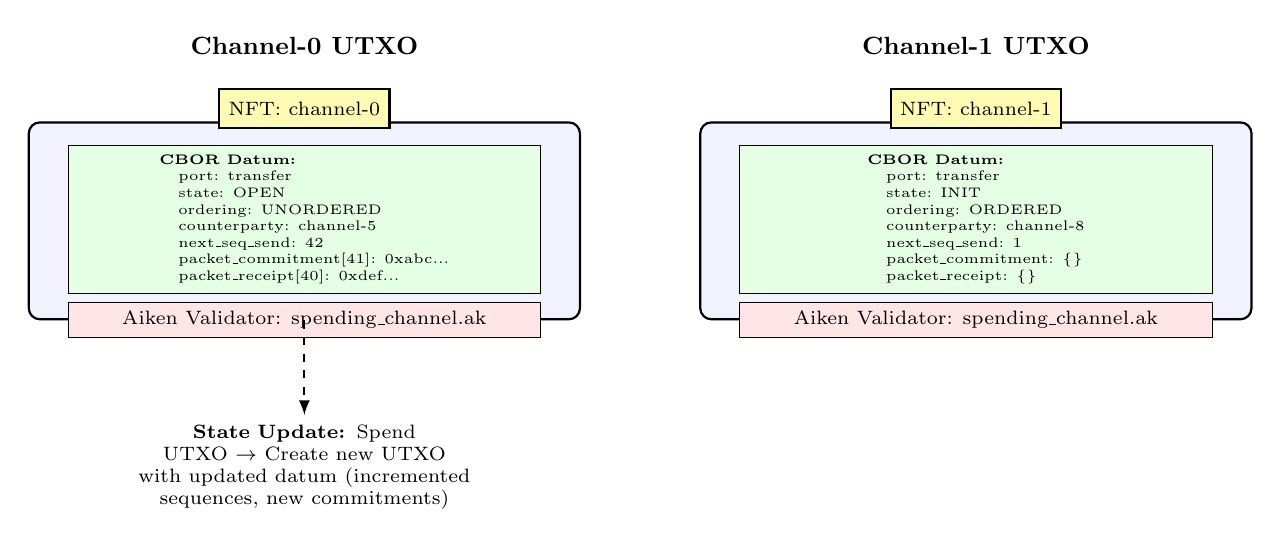
\begin{tikzpicture}[
  node distance=0.6cm,
  utxo/.style={rectangle, draw, thick, rounded corners, align=left, font=\small, minimum width=7cm, minimum height=2.5cm, fill=blue!5},
  nft/.style={rectangle, draw, thick, fill=yellow!30, align=center, font=\scriptsize, minimum width=2cm, minimum height=0.5cm},
  datum/.style={rectangle, draw, fill=green!10, align=left, font=\tiny, minimum width=6cm, minimum height=1.8cm},
  validator/.style={rectangle, draw, fill=red!10, align=center, font=\scriptsize, minimum width=6cm, minimum height=0.4cm},
  arrow/.style={->,>=latex,thick}
]
  % Channel-0 UTXO
  \node[utxo] (utxo0) at (0,0) {};
  \node[nft, above=-0.1cm of utxo0.north] (nft0) {NFT: channel-0};
  \node[datum, below=0.2cm of nft0] (datum0) {
    \textbf{CBOR Datum:}\\
    \quad port: transfer\\
    \quad state: OPEN\\
    \quad ordering: UNORDERED\\
    \quad counterparty: channel-5\\
    \quad next\_seq\_send: 42\\
    \quad packet\_commitment[41]: 0xabc...\\
    \quad packet\_receipt[40]: 0xdef...
  };
  \node[validator, below=0.1cm of datum0] (val0) {Aiken Validator: spending\_channel.ak};
  
  % Channel-1 UTXO
  \node[utxo, right=1.5cm of utxo0] (utxo1) {};
  \node[nft, above=-0.1cm of utxo1.north] (nft1) {NFT: channel-1};
  \node[datum, below=0.2cm of nft1] (datum1) {
    \textbf{CBOR Datum:}\\
    \quad port: transfer\\
    \quad state: INIT\\
    \quad ordering: ORDERED\\
    \quad counterparty: channel-8\\
    \quad next\_seq\_send: 1\\
    \quad packet\_commitment: \{\}\\
    \quad packet\_receipt: \{\}
  };
  \node[validator, below=0.1cm of datum1] (val1) {Aiken Validator: spending\_channel.ak};
  
  % Labels
  \node[above=0.3cm of nft0, font=\small\bfseries] {Channel-0 UTXO};
  \node[above=0.3cm of nft1, font=\small\bfseries] {Channel-1 UTXO};
  
  % Update arrow example
  \node[below=1.2cm of utxo0, font=\scriptsize, text width=6.5cm, align=center] (update) {
    \textbf{State Update:} Spend UTXO $\rightarrow$ Create new UTXO\\
    with updated datum (incremented sequences, new commitments)
  };
  
  \draw[arrow, dashed] (utxo0.south) -- (update.north);
\end{tikzpicture}
\caption{Channel UTXO Architecture: Each IBC channel is represented by a UTXO with an NFT identifier, CBOR-encoded datum containing channel state, and Aiken validator enforcing IBC protocol rules}
\label{fig:channel-utxo}
\end{figure}

The diagram above illustrates how channel state is stored on Cardano using a UTXO-based architecture where each channel is represented by a unique UTXO identified by an NFT token.

\paragraph{Channel UTXO Structure}

Each channel UTXO consists of three key components:

\begin{description}
\item[NFT Token Identifier] A unique NFT token (e.g., \texttt{channel-0}) that identifies the channel's UTXO and enables efficient indexing via Kupo.

\item[CBOR Datum] Contains the complete channel state encoded in CBOR format:
  \begin{itemize}
  \item \textit{Channel metadata}: Port identifier, ordering mode (UNORDERED or ORDERED), connection state (INIT, OPEN, or CLOSED), counterparty channel ID, connection hops, and IBC version
  \item \textit{Sequence counters}: \texttt{next\_sequence\_send}, \texttt{next\_sequence\_recv}, and \texttt{next\_sequence\_ack} for ordered packet processing
  \item \textit{Packet commitments}: Maps from sequence number to commitment hash (\texttt{packet\_commitment[seq]} $\rightarrow$ hash), receipt hash (\texttt{packet\_receipt[seq]} $\rightarrow$ hash), and acknowledgement data (\texttt{packet\_acknowledgement[seq]} $\rightarrow$ ack data)
  \end{itemize}

\item[Aiken Validator] The \texttt{spending\_channel.ak} validator script enforces IBC protocol rules whenever the UTXO is spent or updated, ensuring state transitions comply with the IBC specification.
\end{description}

\paragraph{Multi-Channel Architecture}

Each channel (\texttt{channel-0}, \texttt{channel-1}, etc.) maintains its own independent UTXO with separate state and sequence numbers. This design enables parallel channel operation without state conflicts, as each channel's state is isolated in its own UTXO.

\paragraph{State Update Process}

When a packet is sent, received, or acknowledged, the following transaction flow occurs:

\begin{enumerate}
\item Query Kupo to locate the channel UTXO using its NFT token identifier
\item Parse the current CBOR datum to read channel state and sequence numbers
\item Construct a transaction that spends the current UTXO and creates a new UTXO with updated datum (incremented sequences, new packet commitments)
\item The Aiken validator verifies the state transition follows IBC protocol rules
\item The new UTXO becomes the current canonical channel state
\end{enumerate}

\paragraph{ICS-24 Path Mapping}

This UTXO-based architecture maps naturally to ICS-24 path specifications:

\begin{itemize}
\item \texttt{channelEnds/ports/transfer/channels/channel-0} $\rightarrow$ Find UTXO with NFT \texttt{channel-0} $\rightarrow$ Extract \texttt{datum.state.channel}
\item \texttt{commitments/ports/transfer/channels/channel-0/sequences/58} $\rightarrow$ Find UTXO with NFT \texttt{channel-0} $\rightarrow$ Extract \texttt{datum.state.packet\_commitment[58]}
\end{itemize}

\subsubsection{Design Decision: Single Token Thread (STT) for IBC}
Host
State}\label{design-decision-single-token-thread-stt-for-ibc-host-state}

\paragraph{The Canonical State Problem}

In UTXO-based IBC implementations, we need a way to identify THE canonical IBC host state among potentially many UTXOs. Unlike account-based chains where state naturally lives at a single address with versioning, UTXOs can proliferate, and determining which UTXO represents ``current'' state becomes non-trivial.

\paragraph{Considered Approaches}

\subparagraph{Approach 1: Handler UTXO with AuthToken (Initial Design)}

Store global IBC state (sequence counters, \texttt{ibc\_state\_root}) in a Handler UTXO identified by an authentication token:

\begin{itemize}
\item Query handler script address, filter UTXOs by AuthToken
\item Assume the UTXO with AuthToken is canonical
\item Trust that minting policy prevents duplicate tokens
\end{itemize}

\subparagraph{Issues Identified}

\begin{itemize}
\item \textbf{Ambiguity risk}: If minting policy has a bug or multiple policies exist with same token name, we could have competing Handler UTXOs
\item \textbf{Indexing complexity}: Must query script address, filter through potentially many UTXOs, determine which is ``current''
\item \textbf{No built-in ordering}: Without explicit versioning, difficult to determine which of two Handler UTXOs is newer if both exist
\item \textbf{Race conditions}: If Gateway crashes mid-transaction, unclear which Handler UTXO is canonical when it restarts
\item \textbf{Audit trail}: Tracing state history requires understanding UTXO spending relationships and datum evolution
\end{itemize}

\subparagraph{Approach 2: Single Token Thread (STT) with HostState NFT (Refined Design)}

Use a unique NFT as a linear threading token to enforce canonical state by construction:

\begin{itemize}
\item Mint NFT using one-time policy (consumes specific UTXO reference)
\item HostState UTXO always contains this NFT
\item State updates MUST spend old HostState UTXO and create new one with same NFT
\item STT validator enforces: exactly one output with NFT, version increments by 1
\end{itemize}

\subparagraph{Why This Approach}

The STT design takes advantage of Cardano's blockchain consensus to provide canonical state guarantees by construction: an NFT cannot exist in two unspent UTXOs simultaneously, so the UTXO set contains exactly one unspent output with this NFT at any given slot, eliminating race conditions and indexing ambiguities that would otherwise require sophisticated conflict resolution when multiple Handler UTXOs could theoretically coexist. The NFT acts as a physical token threaded through transactions, where following the NFT through the chain provides the complete, unambiguous state history. There's no need to interpret datum contents or timestamps to determine ordering because the blockchain's spending graph defines the order.

\subparagraph{Version Monotonicity}

The STT validator enforces \texttt{new.version == old.version + 1}, preventing:

\begin{itemize}
\item Replay attacks (cannot resubmit old state)
\item Rollback attacks (cannot go backwards)
\item Parallel forks (only one valid next state)
\end{itemize}

\paragraph{Simplified Operations}

The STT design enables straightforward operations:

\begin{itemize}
\item \textbf{Query}: \texttt{findUtxoByNFT(IBC\_HOST\_STATE)} returns THE canonical state (not ``a'' state)
\item \textbf{Rebuild}: \texttt{queryNFTHistory()} provides complete state evolution
\item \textbf{Audit}: Following the NFT through transactions creates a verifiable state lineage
\end{itemize}

\paragraph{HostState Datum Structure}

\begin{longtable}{p{5cm}p{3cm}p{6cm}}
\toprule
\textbf{Field} & \textbf{Type} & \textbf{Purpose} \\
\midrule
\endfirsthead
\toprule
\textbf{Field} & \textbf{Type} & \textbf{Purpose} \\
\midrule
\endhead
\multicolumn{3}{l}{\textbf{HostState}} \\
\midrule
version & Int & Monotonic counter for version tracking \\
ibc\_state\_root & ByteArray & ICS-23 Merkle root (unchanged from Handler design) \\
next\_client\_sequence & Int & Next available client sequence number \\
next\_connection\_sequence & Int & Next available connection sequence number \\
next\_channel\_sequence & Int & Next available channel sequence number \\
bound\_port & List$<$Int$>$ & List of bound port identifiers \\
last\_update\_time & Int & Unix epoch timestamp for monitoring \\
\midrule
\multicolumn{3}{l}{\textbf{HostStateDatum}} \\
\midrule
state & HostState & The complete host state structure \\
nft\_policy & ByteArray & Must match NFT in UTXO value \\
\bottomrule
\end{longtable}

\textbf{STT Validator Invariants}:

The STT validator enforces five critical invariants when spending the HostState UTXO:

\begin{enumerate}
\item \textbf{Single Input Constraint}: Verify exactly one input contains the NFT (representing old state)
\item \textbf{Single Output Constraint}: Verify exactly one output contains the NFT (representing new state)
\item \textbf{Version Monotonicity}: Verify the version field increments by exactly 1
\item \textbf{State Transition Validity}: Verify the state transition is valid for the operation type (determined by redeemer-based dispatch)
\item \textbf{NFT Policy Consistency}: Verify the NFT policy matches the \texttt{nft\_policy} field in the datum
\end{enumerate}

The validator needs type-specific invariants - CreateClient requires
incrementing \texttt{next\_client\_sequence} while preserving
connection/channel sequences, whereas other operations have different
field constraints. The redeemer acts as a dispatch mechanism so the
validator can branch to operation-specific validation logic.

\textbf{Impact on ICS-23 Proof Infrastructure}:

No difference. The ICS-23 Merkle tree and proof generation logic remains identical. We're only changing: WHERE \texttt{ibc\_state\_root} is
stored (Handler UTXO -\textgreater{} HostState UTXO) - HOW we query it
(AuthToken -\textgreater{} NFT)

The \textasciitilde1000 lines of ICS-23 proof code work unchanged
because the root is still a 32-byte hash over the same IBC state tree
structure.

\subsubsection{Design Decision: Indexer Selection (Kupo vs YACI Store)}\label{design-decision-indexer-selection-kupo-vs-yaci-store}

IBC operations require fast UTXO queries such as "Find all client UTXOs", "Get channel-0 UTXO", and "What was the HostState at height H?". A full Cardano node's chainIndexer is too slow for production use, necessitating an external indexer. The STT HostState architecture significantly simplifies indexing requirements compared to multi-UTXO designs. For current state queries, the indexer simply queries for the single NFT and retrieves the one canonical UTXO, eliminating the need to filter through multiple UTXOs. The NFT itself acts as the index key because Cardano's consensus guarantees that exactly one unspent UTXO can contain a given NFT at any moment, so we don't need complex datum content queries or sophisticated conflict resolution logic. Two primary indexer options were evaluated: Kupo (lightweight, UTXO-focused) and YACI Store (feature-rich, analytics-capable).

\begin{longtable}{p{3.5cm}p{5.5cm}p{5.5cm}}
\toprule
\textbf{Aspect} & \textbf{Kupo (Current Approach)} & \textbf{YACI Store} \\
\midrule
\endfirsthead
\toprule
\textbf{Aspect} & \textbf{Kupo} & \textbf{YACI Store} \\
\midrule
\endhead
\textbf{Description} & Lightweight, fast Cardano chain follower focused on UTXOs & Feature-rich indexer with broader capabilities \\
\midrule
\textbf{Indexing Scope} & UTXOs by address, policy ID, datum hash, asset name & UTXOs, transactions, blocks, stake distributions, metadata \\
\midrule
\textbf{API} & REST API (\texttt{GET /matches/\{pattern\}}) & REST and GraphQL APIs \\
\midrule
\textbf{Storage} & LMDB (no external database) & PostgreSQL database \\
\midrule
\textbf{Resource Footprint} & Minimal ($\sim$2 GB RAM) & Heavier ($\sim$8+ GB RAM) \\
\midrule
\textbf{Deployment} & Single binary, no external dependencies & Requires PostgreSQL, more configuration \\
\midrule
\textbf{NFT Querying} & Excellent (asset name queries) & Supported \\
\midrule
\textbf{Datum Content Search} & No (only datum hash) & Yes (full content indexing) \\
\midrule
\textbf{Historical Queries} & Yes (\texttt{created\_before=\{slot\}}) & Yes (via database queries) \\
\midrule
\textbf{Analytics \& Aggregations} & No & Yes (complex queries, state evolution) \\
\midrule
\textbf{Transaction Context} & UTXO-focused only & Full transaction correlation \\
\midrule
\textbf{Maturity} & Well-maintained by IOG & Newer project, smaller community \\
\midrule
\textbf{Performance} & Fast (in-memory/LMDB) & Potentially slower (database latency) \\
\midrule
\textbf{STT Architecture Fit} & Perfect (NFT-based lookups) & Capable but over-engineered for core needs \\
\midrule
\textbf{Use Case} & Production relay operations & Analytics, dashboards, explorers \\
\bottomrule
\end{longtable}

\textbf{Decision}: Kupo is the recommended choice for MVP and production relay operations due to its lightweight design, perfect alignment with STT's NFT-based architecture, and minimal operational overhead. YACI Store can be added later as a complementary analytics layer if observability requirements emerge, creating a hybrid approach where Kupo handles critical-path queries while YACI Store serves non-critical analytics and user-facing tools. Current implementation uses Kupo integration, with YACI Store evaluation deferred to post-MVP.

\textbf{Governance Integration}:

The Mithril light client has been registered in the sidechain's allowed
clients list. To add support on other Cosmos chains, a governance
proposal must be submitted to update the \texttt{AllowedClients}
parameter to include \texttt{09-mithril} (or the assigned client type
identifier). Once approved, relayers can create Mithril client instances
via \texttt{MsgCreateClient} to establish IBC connections with Cardano.

\textbf{Key Differences from Standard Tendermint Light Clients}:

\begin{enumerate}
\def\labelenumi{\arabic{enumi}.}
\item
  \textbf{Consensus Verification}: Standard Tendermint clients verify
  2/3+ validator signatures on block headers. Mithril clients verify
  aggregate STM signatures from SPOs meeting a stake threshold.
\item
  \textbf{State Storage}: Tendermint uses IAVL Merkle tree with ICS-23
  proofs. Cardano uses UTXO model with CBOR-encoded datums, requiring
  custom path mapping.
\item
  \textbf{Finality}: Tendermint has fast finality (blocks finalized
  immediately). Cardano has probabilistic finality with additional
  confirmation from Mithril certificates (certificate lag).
\item
  \textbf{Proof Structure}: Tendermint proofs contain IAVL Merkle paths.
  Cardano proofs wrap Mithril certificates with transaction Merkle
  proofs and UTXO metadata.
\end{enumerate}

\section{Relayer Foundation}\label{relayer-foundation}

\subsection{ChainHandle Architecture for Cardano Integration}

The Hermes relayer integration for Cardano is built on a plugin architecture using the ChainHandle trait, which defines 57 methods that abstract chain-specific operations. This design allows Hermes core to remain chain-agnostic while delegating Cardano-specific logic (UTXO queries, transaction building, Mithril proof generation, CIP-1852 key derivation) to a dedicated plugin.

The ChainHandle implementation acts as an adapter layer between Hermes's IBC message types and the Cardano Gateway's gRPC API. Each of the 57 methods follows a consistent pattern: translate Hermes types to Gateway protobuf format, make a gRPC call to the Gateway, receive the response, and translate back to Hermes types. This separation of concerns ensures that all Cardano-specific complexity (UTXO indexing via Kupo, transaction building with proper UTXO selection, Aiken validator execution, CBOR datum parsing) is handled by the Gateway, while the ChainHandle remains a thin translation layer.

The architecture is detailed in Section 4.3.1, which documents the full ChainHandle trait interface organized into 13 categories covering lifecycle management, transaction submission, key management, IBC queries (clients, connections, channels, packets), light client building, and proof construction. This modular design provides a clear path to production-grade Cardano IBC relaying without maintaining a relayer fork.



\subsection{Hermes--Gateway Integration}
Architecture}\label{initial-hermesgateway-integration-architecture}
\begin{figure}[H]
\centering
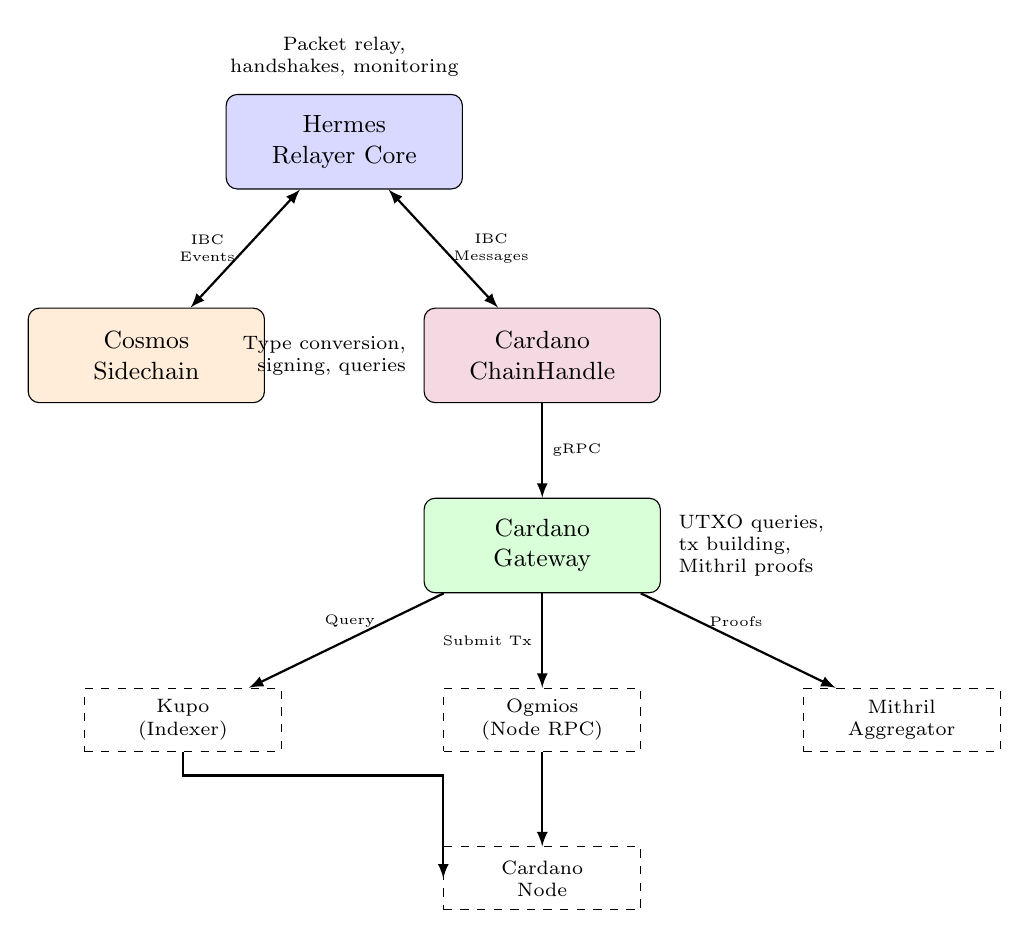
\begin{tikzpicture}[
  node distance=1.2cm and 1.8cm,
  component/.style={rectangle, draw, rounded corners, align=center, font=\small, minimum width=3cm, minimum height=1.2cm},
  infra/.style={rectangle, draw, dashed, align=center, font=\scriptsize, minimum width=2.5cm, minimum height=0.8cm},
  arrow/.style={->,>=latex,thick},
  bidiarrow/.style={<->,>=latex,thick}
]
  % Main components
  \node[component, fill=blue!15] (hermes) {Hermes\\Relayer Core};
  \node[component, fill=orange!15, below left=1.5cm and -0.5cm of hermes] (cosmos) {Cosmos\\Sidechain};
  \node[component, fill=purple!15, below right=1.5cm and -0.5cm of hermes] (chainhandle) {Cardano\\ChainHandle};
  \node[component, fill=green!15, below=of chainhandle] (gateway) {Cardano\\Gateway};
  
  % Infrastructure
  \node[infra, below left=of gateway] (kupo) {Kupo\\(Indexer)};
  \node[infra, below=of gateway] (ogmios) {Ogmios\\(Node RPC)};
  \node[infra, below right=of gateway] (mithril) {Mithril\\Aggregator};
  \node[infra, below=of ogmios] (cardano) {Cardano\\Node};
  
  % Connections
  \draw[bidiarrow] (hermes) -- node[left,font=\tiny,align=center] {IBC\\Events} (cosmos);
  \draw[bidiarrow] (hermes) -- node[right,font=\tiny,align=center] {IBC\\Messages} (chainhandle);
  \draw[arrow] (chainhandle) -- node[right,font=\tiny] {gRPC} (gateway);
  \draw[arrow] (gateway) -- node[left,font=\tiny,pos=0.3] {Query} (kupo);
  \draw[arrow] (gateway) -- node[left,font=\tiny] {Submit Tx} (ogmios);
  \draw[arrow] (gateway) -- node[right,font=\tiny,pos=0.3] {Proofs} (mithril);
  \draw[arrow] (ogmios) -- (cardano);
  \draw[arrow] (kupo.south) -- ++(0,-0.3) -| (cardano.west);
  
  % Labels
  \node[above=0.1cm of hermes, font=\scriptsize, text width=3cm, align=center] {Packet relay,\\handshakes, monitoring};
  \node[left=0.1cm of chainhandle, font=\scriptsize, text width=2.2cm, align=right] {Type conversion,\\signing, queries};
  \node[right=0.1cm of gateway, font=\scriptsize, text width=2.5cm, align=left] {UTXO queries,\\tx building,\\Mithril proofs};
\end{tikzpicture}
\caption{Hermes-Gateway Integration Architecture: Component interaction showing the flow from Hermes relayer through ChainHandle plugin to Cardano infrastructure}
\label{fig:hermes-architecture}
\end{figure}

\textbf{Component Responsibilities}:

\textbf{1. Hermes Relayer (Core)}:
\begin{itemize}
\item Event monitoring via Cosmos websocket and Cardano Gateway polling.
\item Packet lifecycle management (send, receive, acknowledge, timeout).
\item Client update scheduling and execution.
\item Connection and channel handshake orchestration.
\item Metrics and telemetry via Prometheus.
\end{itemize}

\textbf{2. Cardano ChainHandle Plugin}:
\begin{itemize}
\item Implements Hermes's \texttt{ChainHandle} trait for Cardano-specific logic.
\item Translates Hermes IBC types to Gateway protobuf types.
\item Manages Cardano keyring with CIP-1852 derivation.
\item Signs transactions using Ed25519.
\item Queries Gateway for chain state (height, client state, packet commitments).
\item Submits transactions to Gateway for inclusion on Cardano.
\end{itemize}

\textbf{3. Cardano Gateway (NestJS)}:
\begin{itemize}
\item Provides gRPC API implementing standard IBC queries (client, connection, channel, packet).
\item Orchestrates queries to Kupo (UTXO indexer) and Ogmios (Cardano node).
\item Builds unsigned Cardano transactions with proper UTXO selection and balancing.
\item Generates Mithril proofs for state verification on Cosmos.
\item Submits signed transactions to Ogmios for broadcast.
\end{itemize}

\textbf{4. Cardano Infrastructure}:
  \begin{itemize}
\item Cardano Node: Full node for transaction submission and block production.
\item Mithril Aggregator: Provides certificates for light client verification.
\item Kupo: Indexes UTXOs for fast queries by address/datum.
\item Ogmios: JSON-RPC interface to Cardano node.
  \end{itemize}

\textbf{Communication Flow Example} (Packet Relay from Cosmos to Cardano):

\begin{enumerate}
\item Hermes monitors Cosmos for \texttt{SendPacket} events via websocket.
\item Hermes parses event, constructs IBC \texttt{MsgRecvPacket}.
\item Cardano ChainHandle translates \texttt{MsgRecvPacket} to Gateway protobuf format.
\item ChainHandle calls Gateway's \texttt{BuildTransaction} gRPC endpoint with message.
\item Gateway queries Kupo for current channel UTXO.
\item Gateway builds unsigned Cardano transaction updating channel UTXO with packet data.
\item Gateway returns unsigned transaction bytes to ChainHandle.
\item ChainHandle signs transaction using Cardano keyring.
\item ChainHandle calls Gateway's \texttt{SubmitTransaction} gRPC endpoint with signed transaction.
\item Gateway submits transaction to Ogmios.
\item Ogmios broadcasts transaction to Cardano network.
\item Hermes waits for transaction confirmation (monitors Gateway's height endpoint).
\item Once confirmed, Hermes emits \texttt{WriteAcknowledgement} event on Cardano.
\item Hermes constructs \texttt{MsgAcknowledgement} for Cosmos.
\item Cosmos sidechain verifies Mithril proof and processes acknowledgement.
\end{enumerate}

\textbf{Current Implementation Status}:
  \begin{itemize}
\item [DONE] Gateway gRPC API complete and tested.
\item [DONE] ChainHandle trait scaffolding complete.
\item [IN-PROGRESS] ChainHandle gRPC client implementation in progress (basic queries done, transaction submission pending).
\item [IN-PROGRESS] Keyring CIP-1852 derivation stubbed (needs BIP32 library integration).
\item [IN-PROGRESS] Transaction signer CBOR parsing stubbed (needs cardano-serialization-lib integration).
\item [PENDING] End-to-end integration testing blocked on ChainHandle completion.
  \end{itemize}

\section{Conclusion}\label{conclusion}

\textbf{Milestone 2 Deliverables Summary}:

  \begin{itemize}
\item Codebase audit complete with strengths, weaknesses, and recommendations identified.
\item Documentation gaps catalogued and prioritized, as well as known issues and gaps.
\item Cosmos SDK/ibc-go v10.x compatibility assessed with clear migration paths.
\item ADR on Hermes migration strategy drafted, detailed explanation on ChainHandle concept (Section 4).
\item Light client designs for both Cardano and Mithril documented with ICS-23 verification logic (Limitations documented with respect to UTXO inclusion and exclusion proofs, which are in theory a bottleneck for ICS-23)
\item Hermes relayer integration architecture defined, with scaffolding complete and implementation in progress.
  \end{itemize}

\end{document}
